\newpage

\section*{Support Information}
\addcontentsline{toc}{section}{Support Information}

\subsection*{All stop words used in this project}

\{'', 'november', 'shouldn', 'necessary', 'inc', 'twice', 'whether', 'from', "you'll", 'aspect', 'proposed', 'measure', 'as', 'significant', 'took', 'w', 't', 'his', 'thru', 'almost', 'proposal', 'vi', 'out', 'say', 'someone', 'd', 'www', "didn't", 'mostly', 'gone', 'edu', 'f', 'never', 'h', 'chinese', 'october', 'down', 'hither', 'those', 'serious', 'specific', 'our', 'is', 'are', "you've", 'poorly', 'himself', 'program', 'i', 'become', 'awfully', 'o', 'something', 'near', 'come', 'detected', 'pursue', 'less', 'february', 'able', 'consider', 'just', 'gotten', 'until', 'going', 'changes', 'nine', 'away', 'three', 'unless', 'somebody', 'zero', 'progress', 'doi', 'like', 'upon', 'although', 'seemed', 'together', "it's", 'enable', 'behind', 'recent', 'e', 'itself', 'august', 'because', "isn't", 'iv', 'far', 'considering', 'often', 'made', 'therein', 'indeed', 'need', "shan't", 'x', 'inasmuch', 'all', 'so', 'same', 'rather', 'obviously', 'others', 'no', 'theirs', 'associated', 'l', 'thoroughly', "that'll", 'four', 'beside', 'thereby', 'needed', 'herself', 'training', 'latter', 'let', 'knows', 'main', 'exactly', 'aren', 'third', 'following', 'linkage', 're', 'beyond', 'enough', 'thats', 'not', 'll', 'application', 'got', 'lately', 'herein', 'respectively', 'cover', 'lest', "couldn't", 'but', 'value', 'focus', 'before', 'large', 'he', 'seem', 'insofar', 'truly', 'english', 'do', 'yourself', 'nor', 'beforehand', 'vii', 'toward', 'certainly', 'containing', 'second', 'been', 'sure', 'academic', 'q', 'ought', 'applicant', 'willing', 'example', 'about', 'becoming', 'currently', 'between', 'everything', 'liked', 'very', 'many', 'study', 'one', 'anyhow', 'across', 'relate', 'etc', 'forth', 'seeming', 'hopefully', 'aim', 'km', 'next', 'specifying', 'tell', 'during', 'increase', 'since', 'fifth', 'still', 'plus', 'against', 'though', 'small', 'quite', 'durham', 'oh', 'certain', 'approach', 'baseoxford', 'too', 'name', 'causes', 'theres', 'such', 'after', 'course', 'through', 'count', 'might', 'indicates', 'neither', 'future', 'examine', 'face', 'five', 'either', 'k', 'bed', 'nobody', 'wherever', 'had', 'cannot', 'kept', 'concerning', 'formerly', 'here', 'go', 'once', 'way', 'understand', 'lead', 'available', 'however', 'uses', 'alone', 'specify', 'well', 'whither', 'off', 'easily', 'last', 'thanx', 'whereby', 'below', 'immediate', 'please', 'how', 'at', 's', 'taken', "needn't", 'a', 'without', 'then', 'only', 'induce', 'seen', 'ourselves', 'six', 'http', 'take', 'further', 'give', 'moreover', 'africa', 'reasonably', 'wasn', 'least', 'okay', 'unlikely', 'everyone', 'known', 'myself', 'afterwards', 'elsewhere', 'seven', 'therefore', 'contains', "don't", 'needn', 'later', 'local', 'according', 'she', 'good', 'most', 'little', 'which', 'closely', 'highly', 'see', 'sup', 'comes', 'much', '\_', 'important', 'anyone', 'japanese', 'getting', 'recently', 'always', 'p', 'david', 'ok', 'using', 'et', 'somewhat', 'entirely', 'ma', 'became', "you'd", 'dataset', 'continued', 'c', 'field', 'they', 'great', 'sometime', 'trying', 'essential', 'work', 'won', 'mustn', 'relatively', 'look', 'know', 'along', 'amongst', 'apart', 'west', 'now', 'possible', 'somewhere', 'seeing', 'definitely', 'descriptionabstract', 'viz', 'have', 'within', 'tried', 'overall project summary', 'throughout', 'any', 'nothing', 'test', 'perhaps', 'programme', 'my', 'march', 'under', 'better', 'given', 'whole', 'sheet', 'thereafter', 'goes', 'shan', 'sensible', 'channel', 'and', 'in', 'consequently', 'asking', 'each', 'greetings', 'description provided by applicant:', 'december', 'july', 'anything', 'onto', 'isn', 'extend', 'whereupon', 'having', 'to', 'vast', 'lt', 'likely', 'while', 'inward', 'meanwhile', 'april', 'hereby', 'usually', 'you', 'co', 'than', 'survey', 'why', 'be', 'outside', 'even', 'different', 'we', 'develop', 'also', 'knowledge', 'howbeit', 'successful', 'provides', 'indicated', 'y', 'nowhere', 'normally', 'went', 'whenever', 'whereas', 'investigate', 'un', 'hers', 'soon', 'affect', 'range', 'first', 'think', 'believe', 'award', 'seriously', 'latterly', 'particular', 'questions', 've', 'them', 'instead', 'secondly', 'whereafter', 'th', 'other', 'was', 'project description', 'india', 'hello', 'mainly', 'used', 'by', 'anybody', 'whatever', 'done', 'needs', 'help', 'whoever', 'various', 'this', 'couldn', 'above', 'r', 'did', "doesn't", 'cell', 'does', 'gets', 'decide', 'follows', 'somehow', 'namely', 'there', 'unto', 'haven', 'another', 'include', 'september', 'description', 'hi', 'line', 'more', 'maybe', "hasn't", 'came', 'says', 'based', 'besides', 'nevertheless', 'cause', 'g', 'thus', 'don', 'with', 'placed', 'should', 'due', 'doing', 'specified', 'own', 'yes', 'among', 'mightn', 'themselves', 'ignored', 'sorry', 'again', "shouldn't", 'nice', 'saw', 'anyway', "hadn't", "mustn't", 'june', 'show', 'successfully', 'yours', 'mean', 'right', 'contain', 'students', 'especially', 'shall', 'underly', 'china', 'its', 'can', 'looks', 'everybody', "weren't", 'ms', 'clearly', 'us', 'hence', 'anywhere', 'hasn', 'selves', 'brief', 'ltd', 'tries', 'inner', 'up', 'appear', 'sent', 'remains', 'big', 'provide', 'an', 'use', 'around', "wasn't", 'except', 'regarding', 'for', 'probably', 'receive', 'uk', 'appropriate', 'sector', "you're", 'their', 'method', 'appreciate', 'south', 'presumably', 'could', 'want', 'b', 'greatly', 'get', 'ii', 'few', "should've", 'u', 'the', 'really', 'didn', 'apply', 'hadn', 'research', 'some', 'project', 'seems', 'her', 'looking', 'tends', 'becomes', 'furthermore', 'nearly', 'despite', 'goal', 'may', 'towards', 'funded', 'ex', 'unfortunately', 'support', 'thanks', 'cant', 'try', 'none', 'whom', 'into', 'former', 'me', 'thereupon', 'ask', 'happens', 'keep', 'said', "haven't", 'thence', 'hardly', 'doesn', 'wherein', 'downwards', 'merely', 'call', 'british', 'two', 'm', 'whence', 'seminar', 'on', 'z', 'sometimes', 'yet', 'these', 'com', 'where', 'several', 'london', 'yourselves', 'subject', 'nd', 'qv', 'both', 'corresponding', 'org', 'input', 'rd', 'new', 'dr', 'otherwise', 'purpose', 'your', 'would', 'everywhere', 'best', 'particularly', 'thorough', 'make', 'supports', 'regards', "she's", 'sub', 'predict', 'area', 'actually', 'wonder', 'being', 'easy', 'lack', 'propose', 'must', 'ie', 'easet', 'data', 'him', 'will', 'thank', 'hereupon', 'wouldn', 'hereafter', 'has', 'abstract', 'of', 'https', 'indicate', 'per', 'worldwide', 'regardless', 'que', 'shown', "aren't", 'that', 'north', "wouldn't", 'vs', 'over', 'whose', 'model', 'areas', 'novel', 'weren', 'uucp', 'when', 'useful', 'gives', 'every', 'ones', 'january', 'were', 'high', 'described', 'v', "mightn't", 'accordingly', 'unique', 'n', 'old', 'am', 'ours', 'if', 'what', 'already', 'or', 'iii', 'else', 'objective', 'function', 'eg', 'anyways', 'followed', 'summary', "won't", 'it', 'estimate', 'j', 'allow', 'summaryabstract', 'saying', 'require', 'lot', 'non', 'ain', 'funding', 'overall', 'keeps', 'amountdetail', 'contact', 'wants', 'run', 'identify', 'ever', 'viii', 'self', 'experience', 'who', 'wish', 'via', 'eight', 'noone', 'aside', 'welcome', 'participation' \}

\subsection*{Topic Similarity and Model Stability}

To explore how the two topics in two sub-models at the same k-topic model differ from each other. I calculated Jensen-Shannon Divergence (JSD) between best-matched topic pairs since it has been proven to outperform other divergence-based similarity metrics \cite{Kim2011}. Due to the stochasticity of the LDA model, topics with similar words won't be in the same order between sub-models with different random states. I applied the Kuhn-Munkres algorithm in the 'scipy' package in Python \cite{scipy}, also known as the Hungarian algorithm, in order to solve this minimum weight bipartite matching problem \cite{hungarian}. Afterwards, the JSD distance between two best-matched topics from two different sub-models of a k-topic model (see Section 2.5 Model Selection) can be calculated by using the 'Gensim' package in Python \cite{gensim}. Then, from these calculated distances between topics, the averaged $similarity$ between two sub-models in the same k-topic model can be expressed as follows:

\begin{equation}
  Sim(M^k_u, M^k_v) = \frac{1}{k} \sum^k_{x=1}JSD(Z_{ux}, \phi(Z_{vx}))
\end{equation}

where $M^k_u$ and $M^k_v$ are $u-th$ and $v-th$ sub-models in the model set with the topic indicator $k$; $JSD(Z_{ux}, \phi(Z_{ux}))$ are the JSD measure between the best-matched topics $Z_{ix}$ and $\phi(Z_{ix})$, where $Z_{ix}$ is the $x-th$ topic in $M^k_u$ and $\phi(Z_{ux})$ is the most similar topic (i.e. best-matched) with $Z_{ux}$ in $M^k_v$.

Afterwards, the $stability$ between two k-topic models is expressed as:

\begin{equation}
  Stab(M^k) = \frac{2}{n \times (n-1)} \sum^r_{u,v,u<v} Sim(M^k_u, M^k_v)
\end{equation}

where $n$ is the number of sub-models in a single k-topic model, which is 10 in my project. The topic model with the lowest $stability$ and median $similarity$ of pair-wise sub-models are considered as my final topic model.

\subsection*{Hierarchical Clustering}

To explore how similar topics change with different funding agencies and funding amounts. The hierarchical clustering with the Ward linkage method, known as the minimal increase of sum-of-squares (MISSQ), is applied for clustering similar topics. Ward linkage are more explicable way to cluster noisy data \cite{ward2}. The distance between two clusters can be calculated by the sum of squares of the deviations from mean or the centroid (i.e. the error of sum squares or ESS)\cite{ward}. The Ward approach tries to find the minimal increase of ESS at every iteration. The distance between clusters using the Ward approach can be expressed as \cite{ward2}:

\begin{equation}
  Dist(X, Y) = ESS(X \cup Y) - [ESS(X) + ESS(Y)]
\end{equation}

where $X$, $Y$ are two different clusters, $X \cup Y$ is a combined cluster of X and Y.

\subsection*{Topic Label Assignment}

To assign more interpretable labels for topics derived from the LDA model, pyLDAvis is utilised, which is a Python package providing a method of interactive visualisation for the LDA model \cite{LDAvis}. In the approach, the $relevance$ measure of words of topics is defined, allowing to rank topic terms by not only the probability under a topic but also its lift. The $relevance$ can be described as \cite{LDAvis}:

\begin{equation}
  r(w,k|\lambda) = \lambda log(\phi_{kw}) + (1+\lambda)log(\frac{\phi_{kw}}{p_w})
\end{equation}

where $\phi_{kw}$ is the probability of a word $w$ for topic k, $p_w$ is defined as the marginal probability of term $w$, $\lambda$ ($0 \leq \lambda \leq 1$) is a parameter that can tune the weight between logged probability ($\phi_{kw}$) and its logged lift ($\frac{\phi_{kw}}{p_w}$). If topic terms are ranked by only logged probability estimated by the LDA model, it could affect interpretability of topics due to globally frequent tokens; if the topic terms are ranked by solely the $lift$, which could weaken the impact of globally frequent tokens but also could result in uninterpretable rare words \cite{taddy2011estimation}. Hence, a suitable $\lambda$ value can give a solution for the problem of the non-interpretability of topics brought by either globally frequent words or field-specialised terminologies.

\subsection*{Topic Inference of the LDA Model}

Two common approaches are utilised to infer the coefficients for document-topic and topic-word matrices \cite{gibbs_lda}: variational Bayesian approach and collapsed Gibbs sampling approach. The former method is a variational Bayesian method with an Expectation-Maximization (EM) algorithm proposed by Blei et al. (2003) \cite{LDA} in their original paper of the LDA model. By the variational approach, the computational process is faster but may produce inaccurate inferences \cite{jordan1999}. The latter approach is to use collapsed Gibbs sampling to infer the coefficients of matrices, which is introduced by Griffiths and Steyvers(2004). For this method, theoretically, the accuracy of inference can be improved but with the cost of more intensive computation, which could therefore affect the efficiency of the model as the size of datasets are larger \cite{gibbs_lda}.

\subsection*{Topic space and top-30 words of eight topics by pyLDAvis}

\begin{figure}[H]
    \centering
    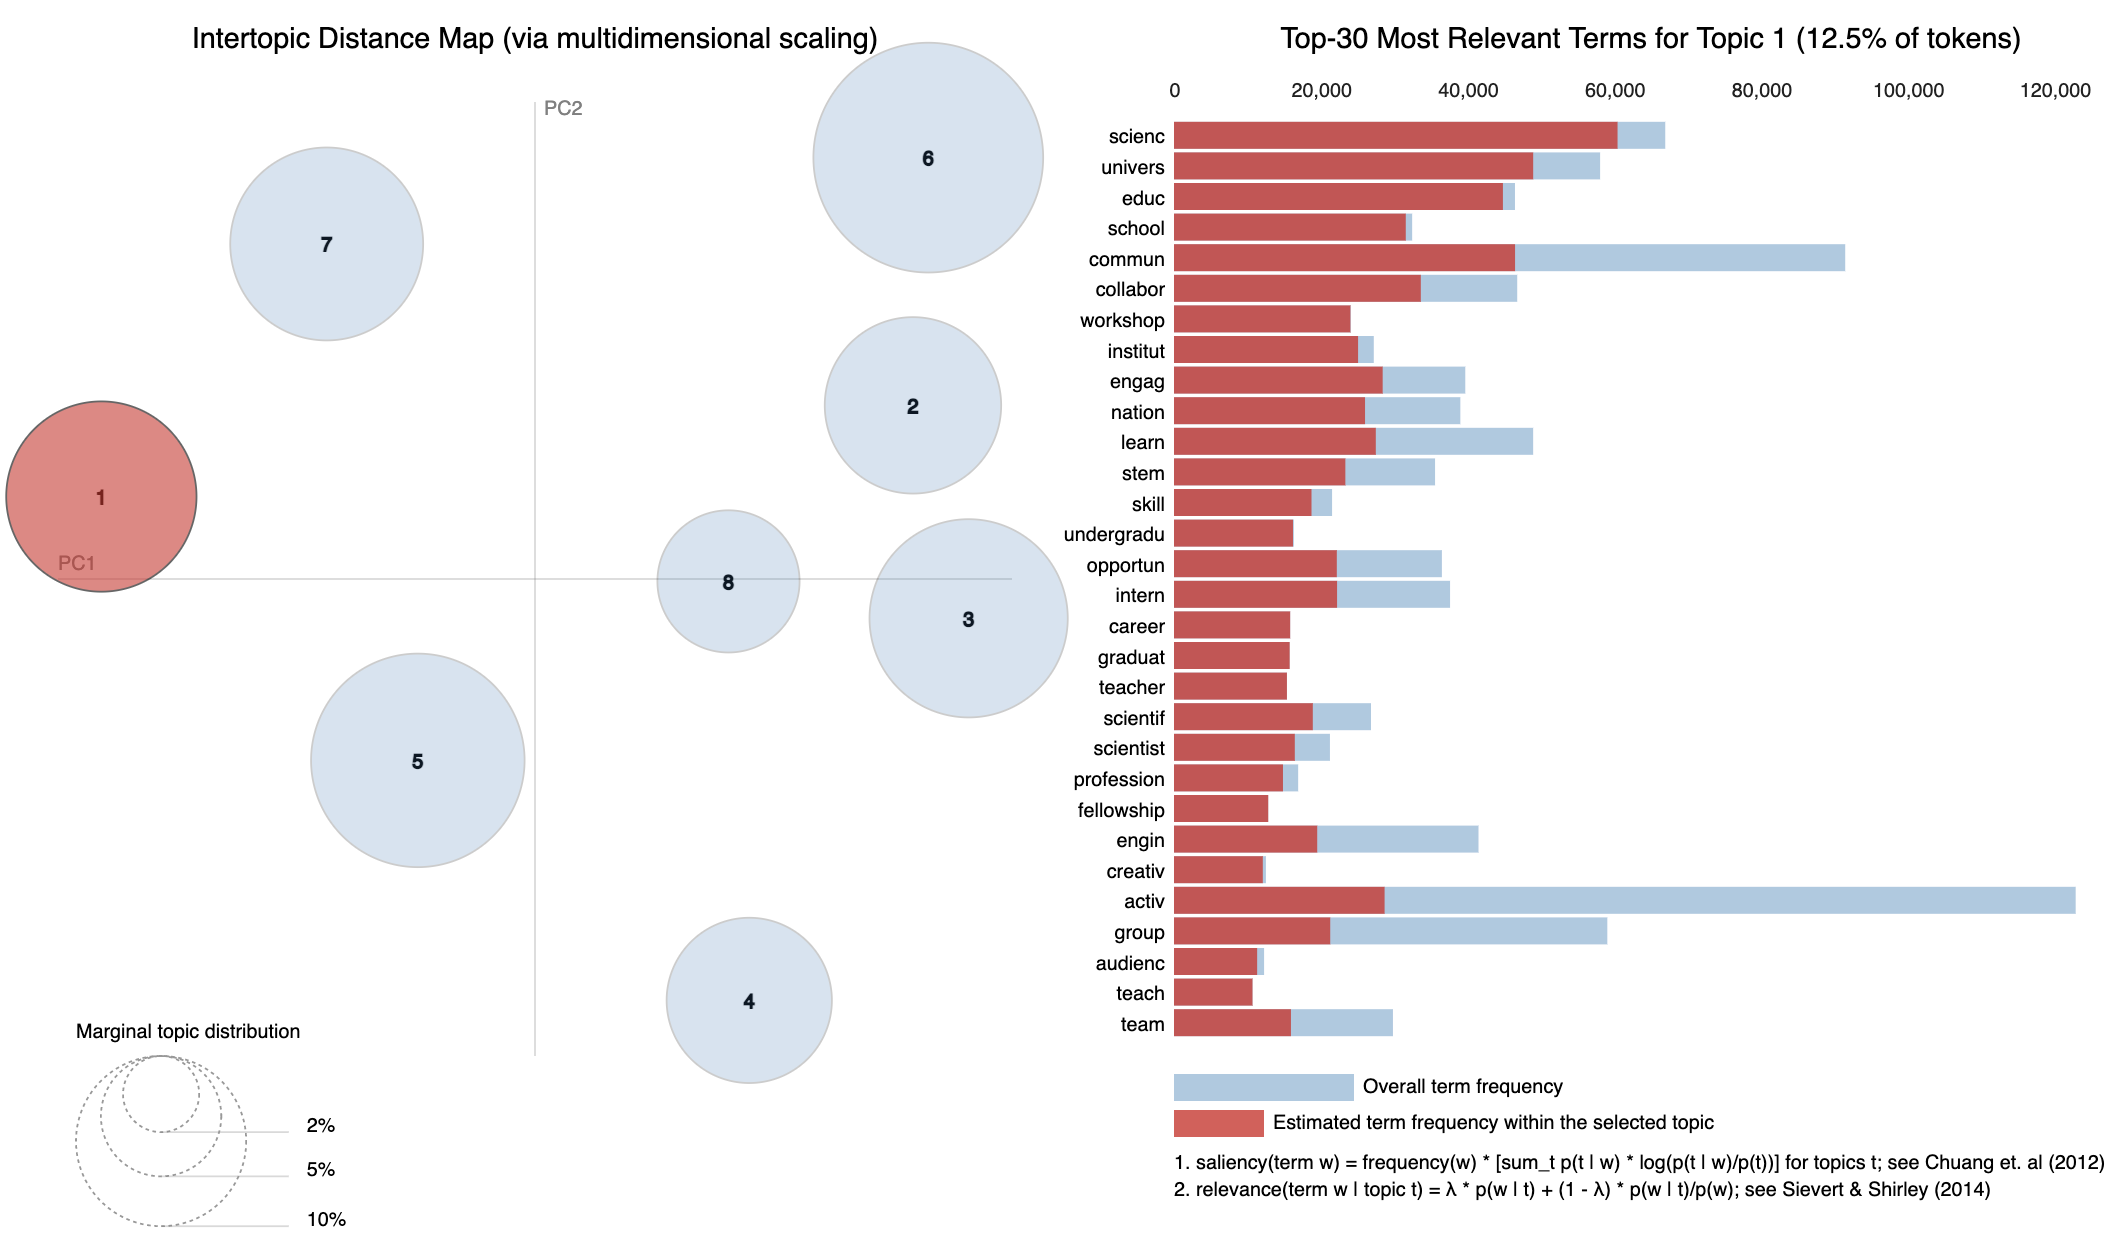
\includegraphics[width = 16cm, height = 10cm]{./img/LDAvis.png}
    \caption{Visualisation of topic 1 by pyLDAvis}
\end{figure}

\begin{figure}[H]
    \centering
    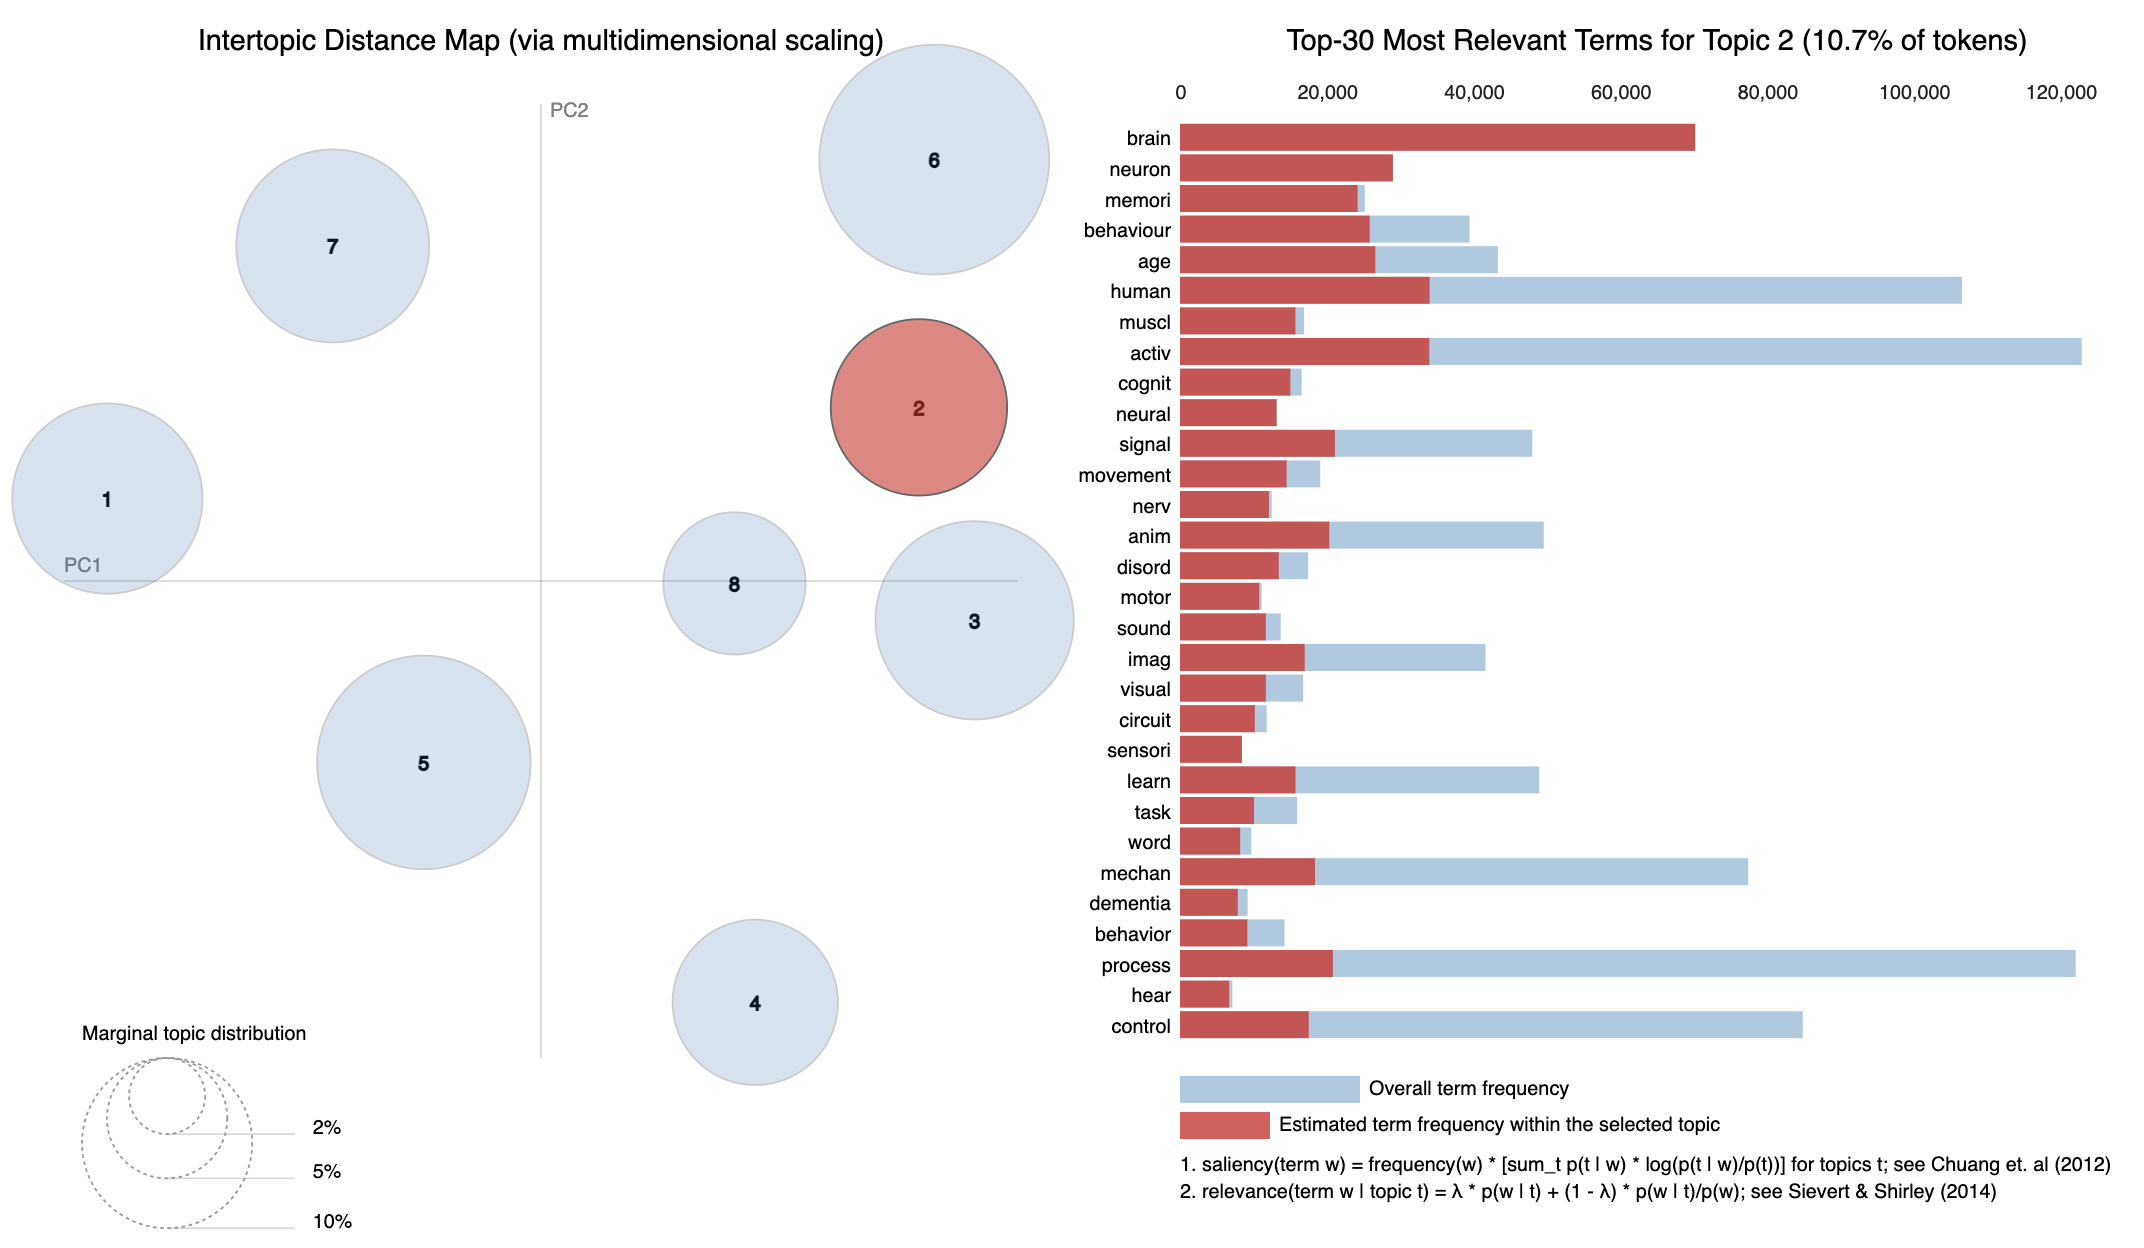
\includegraphics[width = 16cm, height = 10cm]{./img/pylda_topic2.png}
    \caption{Visualisation of topic 2 by pyLDAvis}
\end{figure}

\begin{figure}[H]
    \centering
    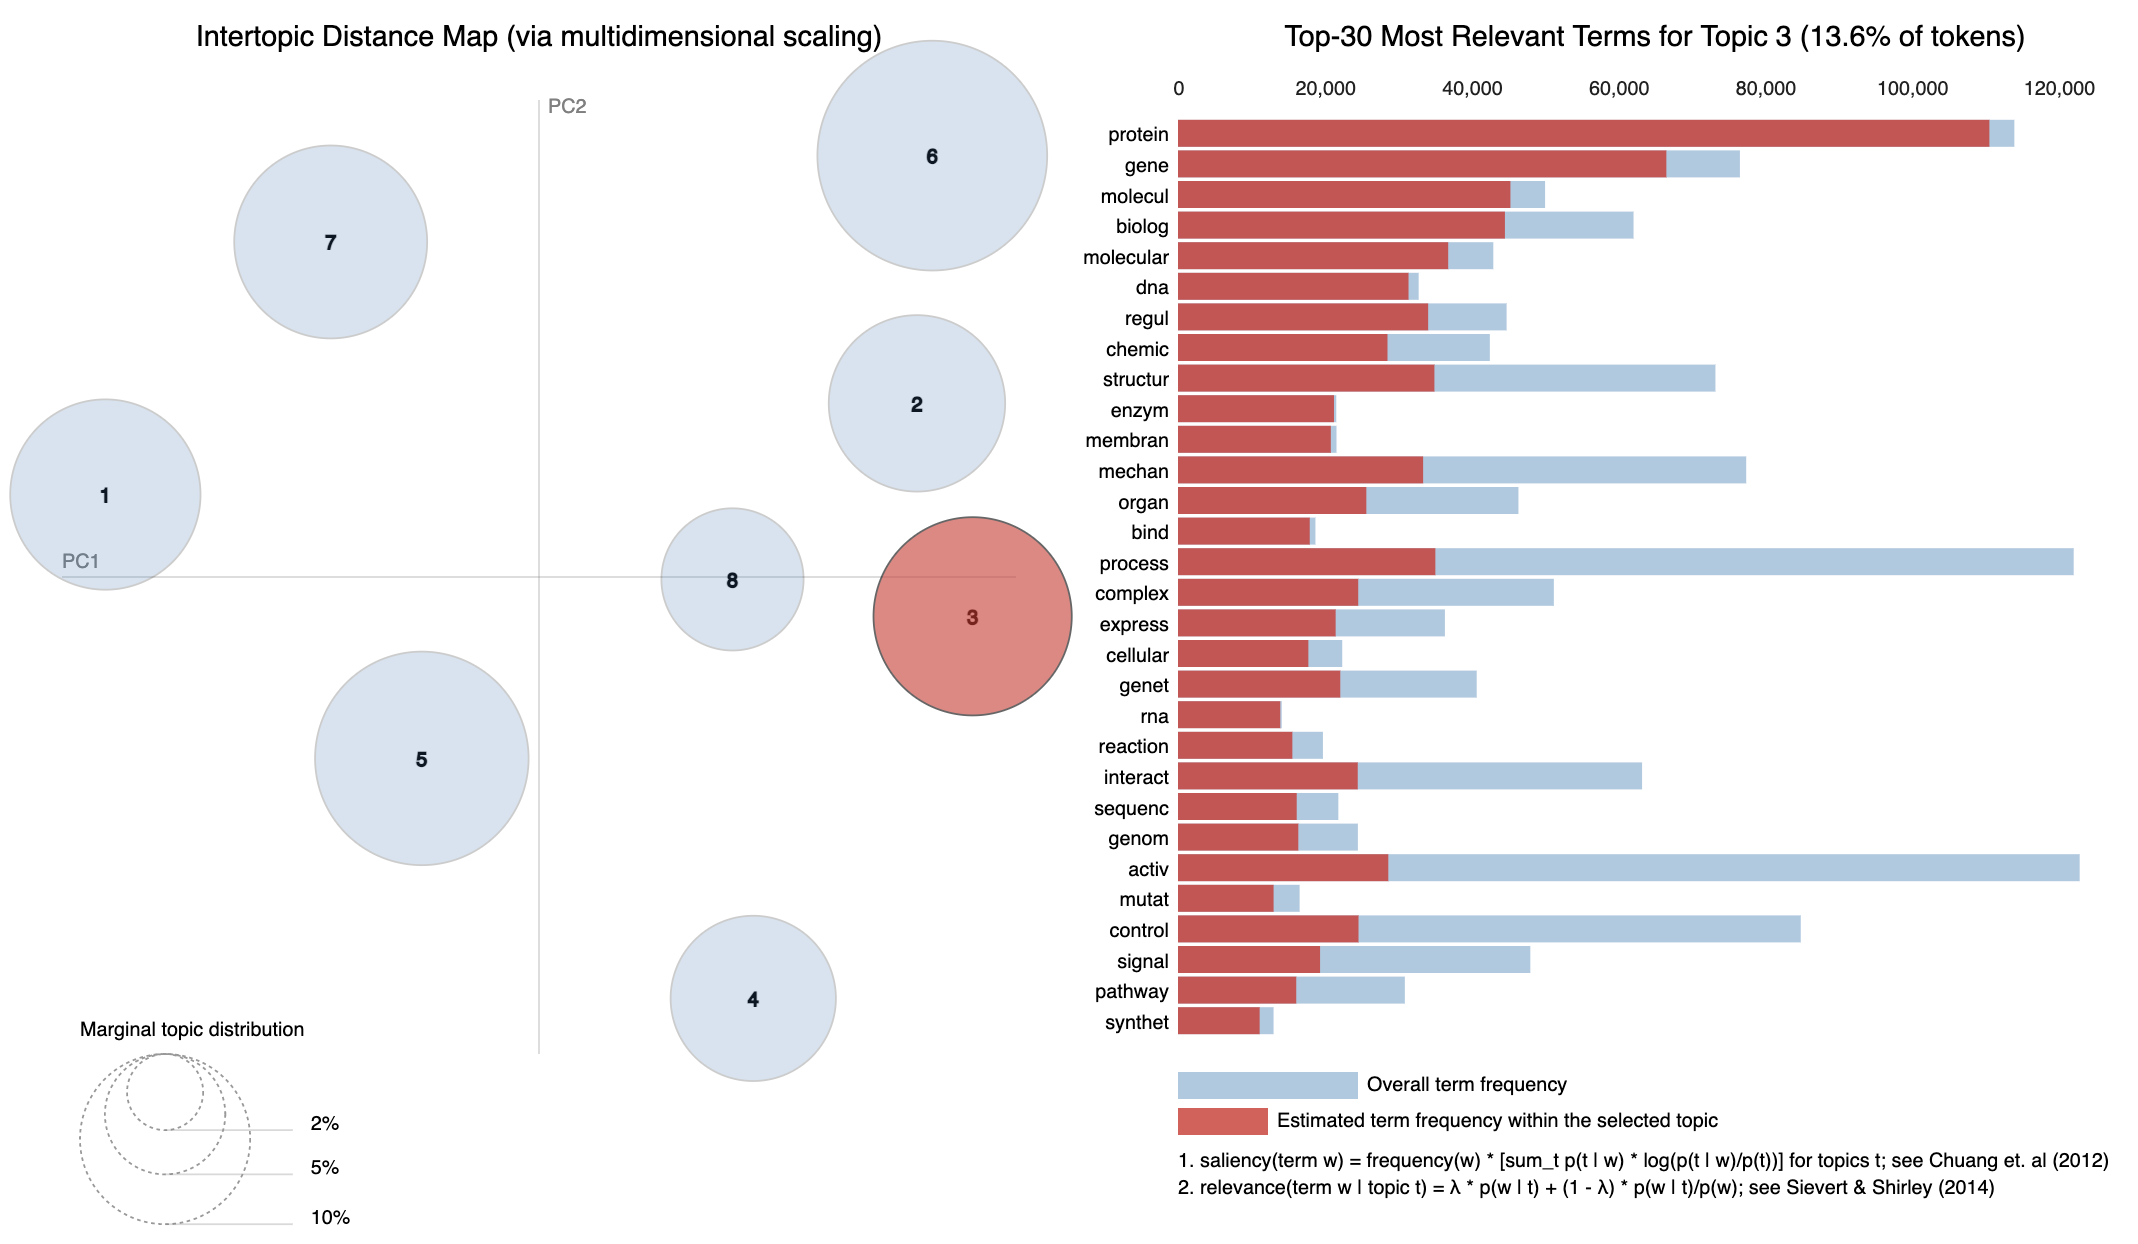
\includegraphics[width = 16cm, height = 10cm]{./img/pylda_topic3.png}
    \caption{Visualisation of topic 3 by pyLDAvis}
\end{figure}

\begin{figure}[H]
    \centering
    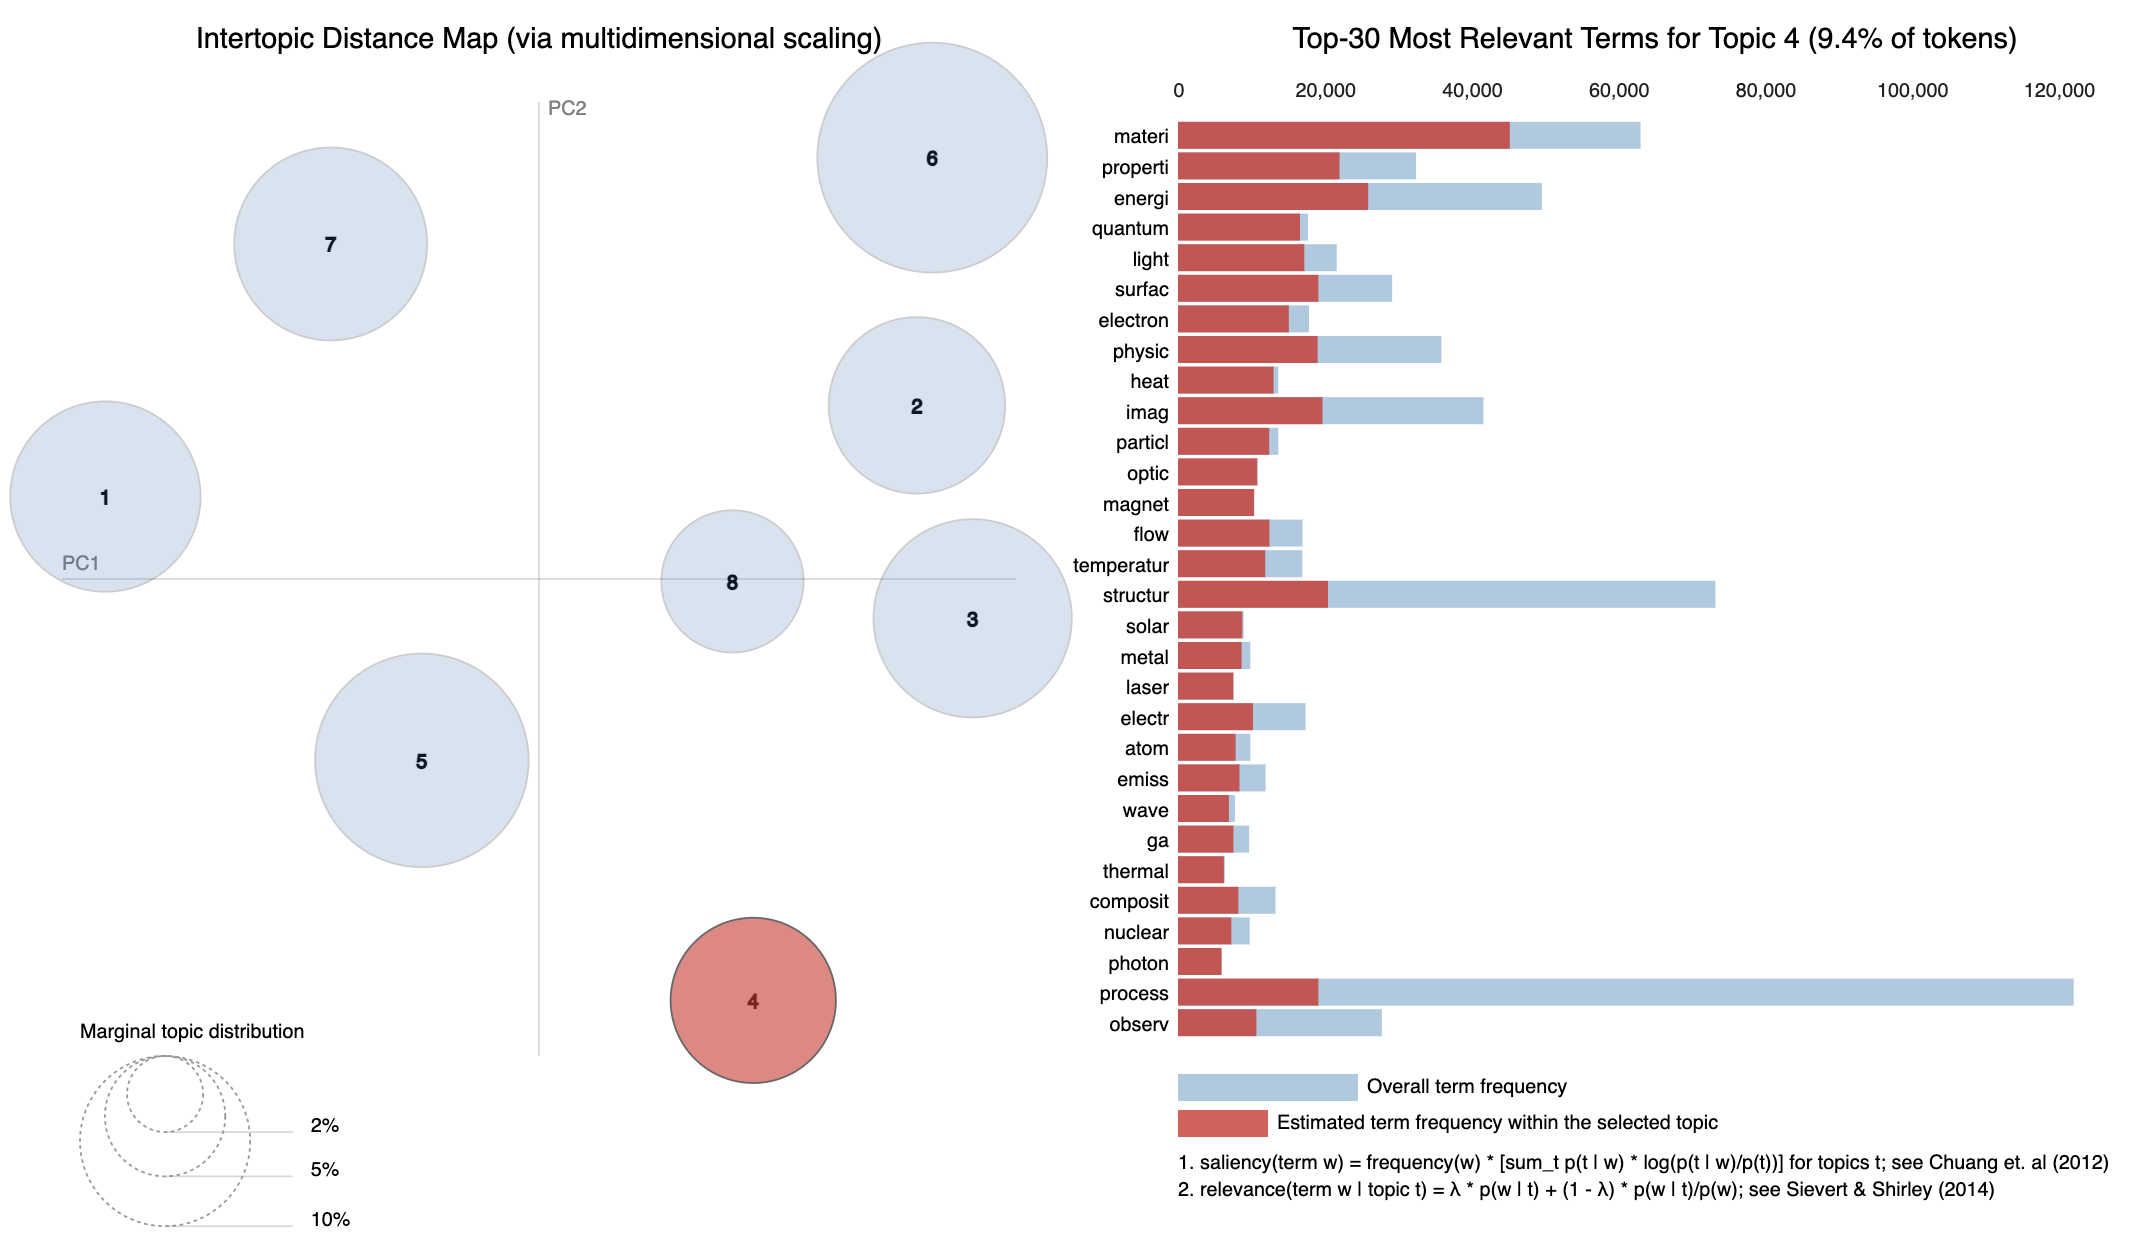
\includegraphics[width = 16cm, height = 10cm]{./img/pylda_topic4.png}
    \caption{Visualisation of topic 4 by pyLDAvis}
\end{figure}


\begin{figure}[H]
    \centering
    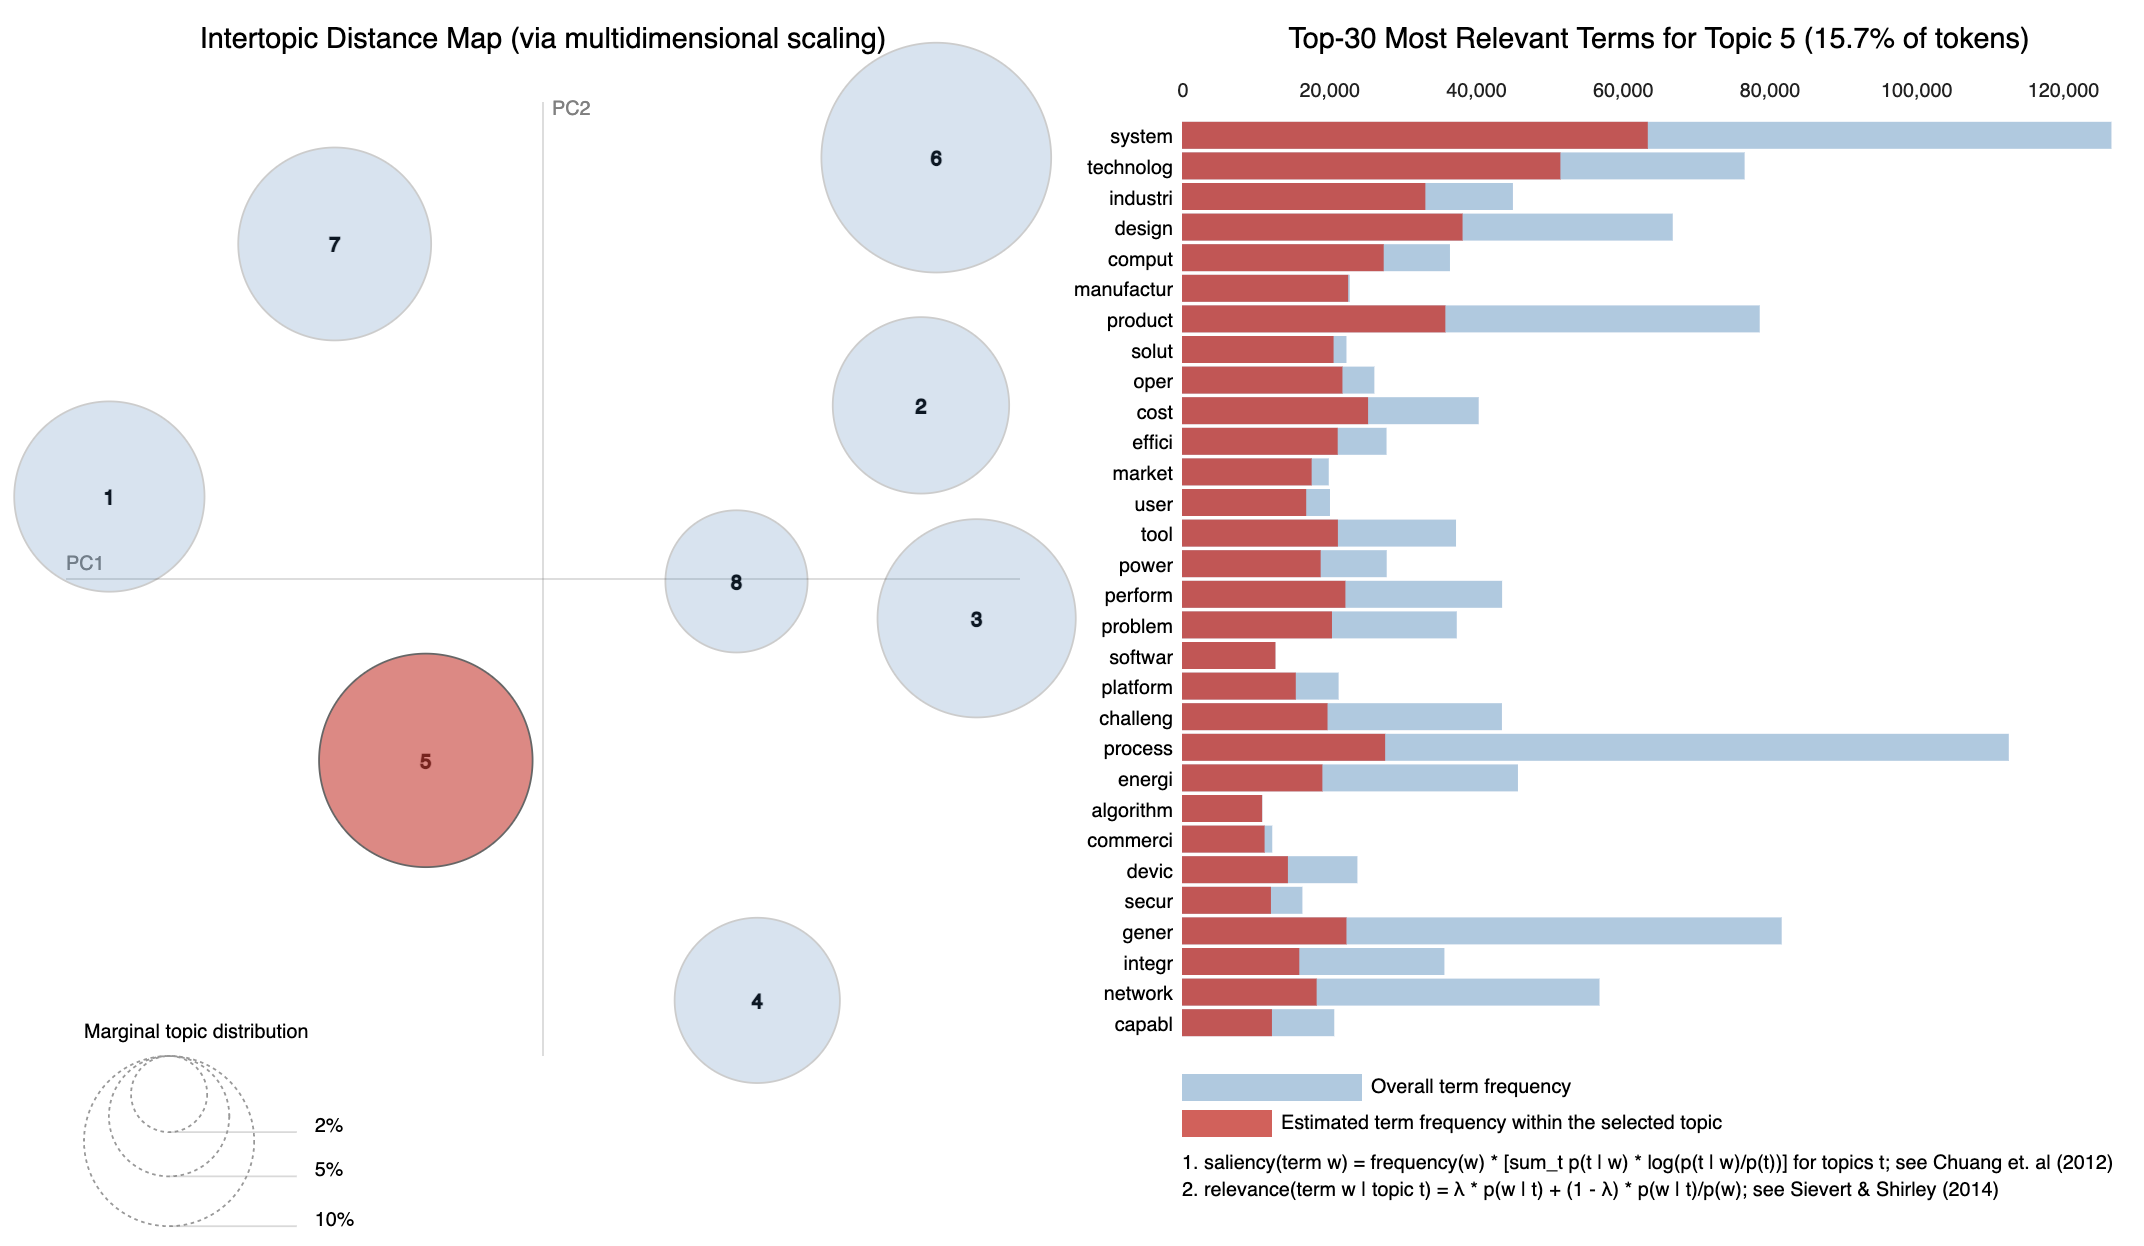
\includegraphics[width = 16cm, height = 10cm]{./img/pylda_topic5.png}
    \caption{Visualisation of topic 5 by pyLDAvis}
\end{figure}


\begin{figure}[H]
    \centering
    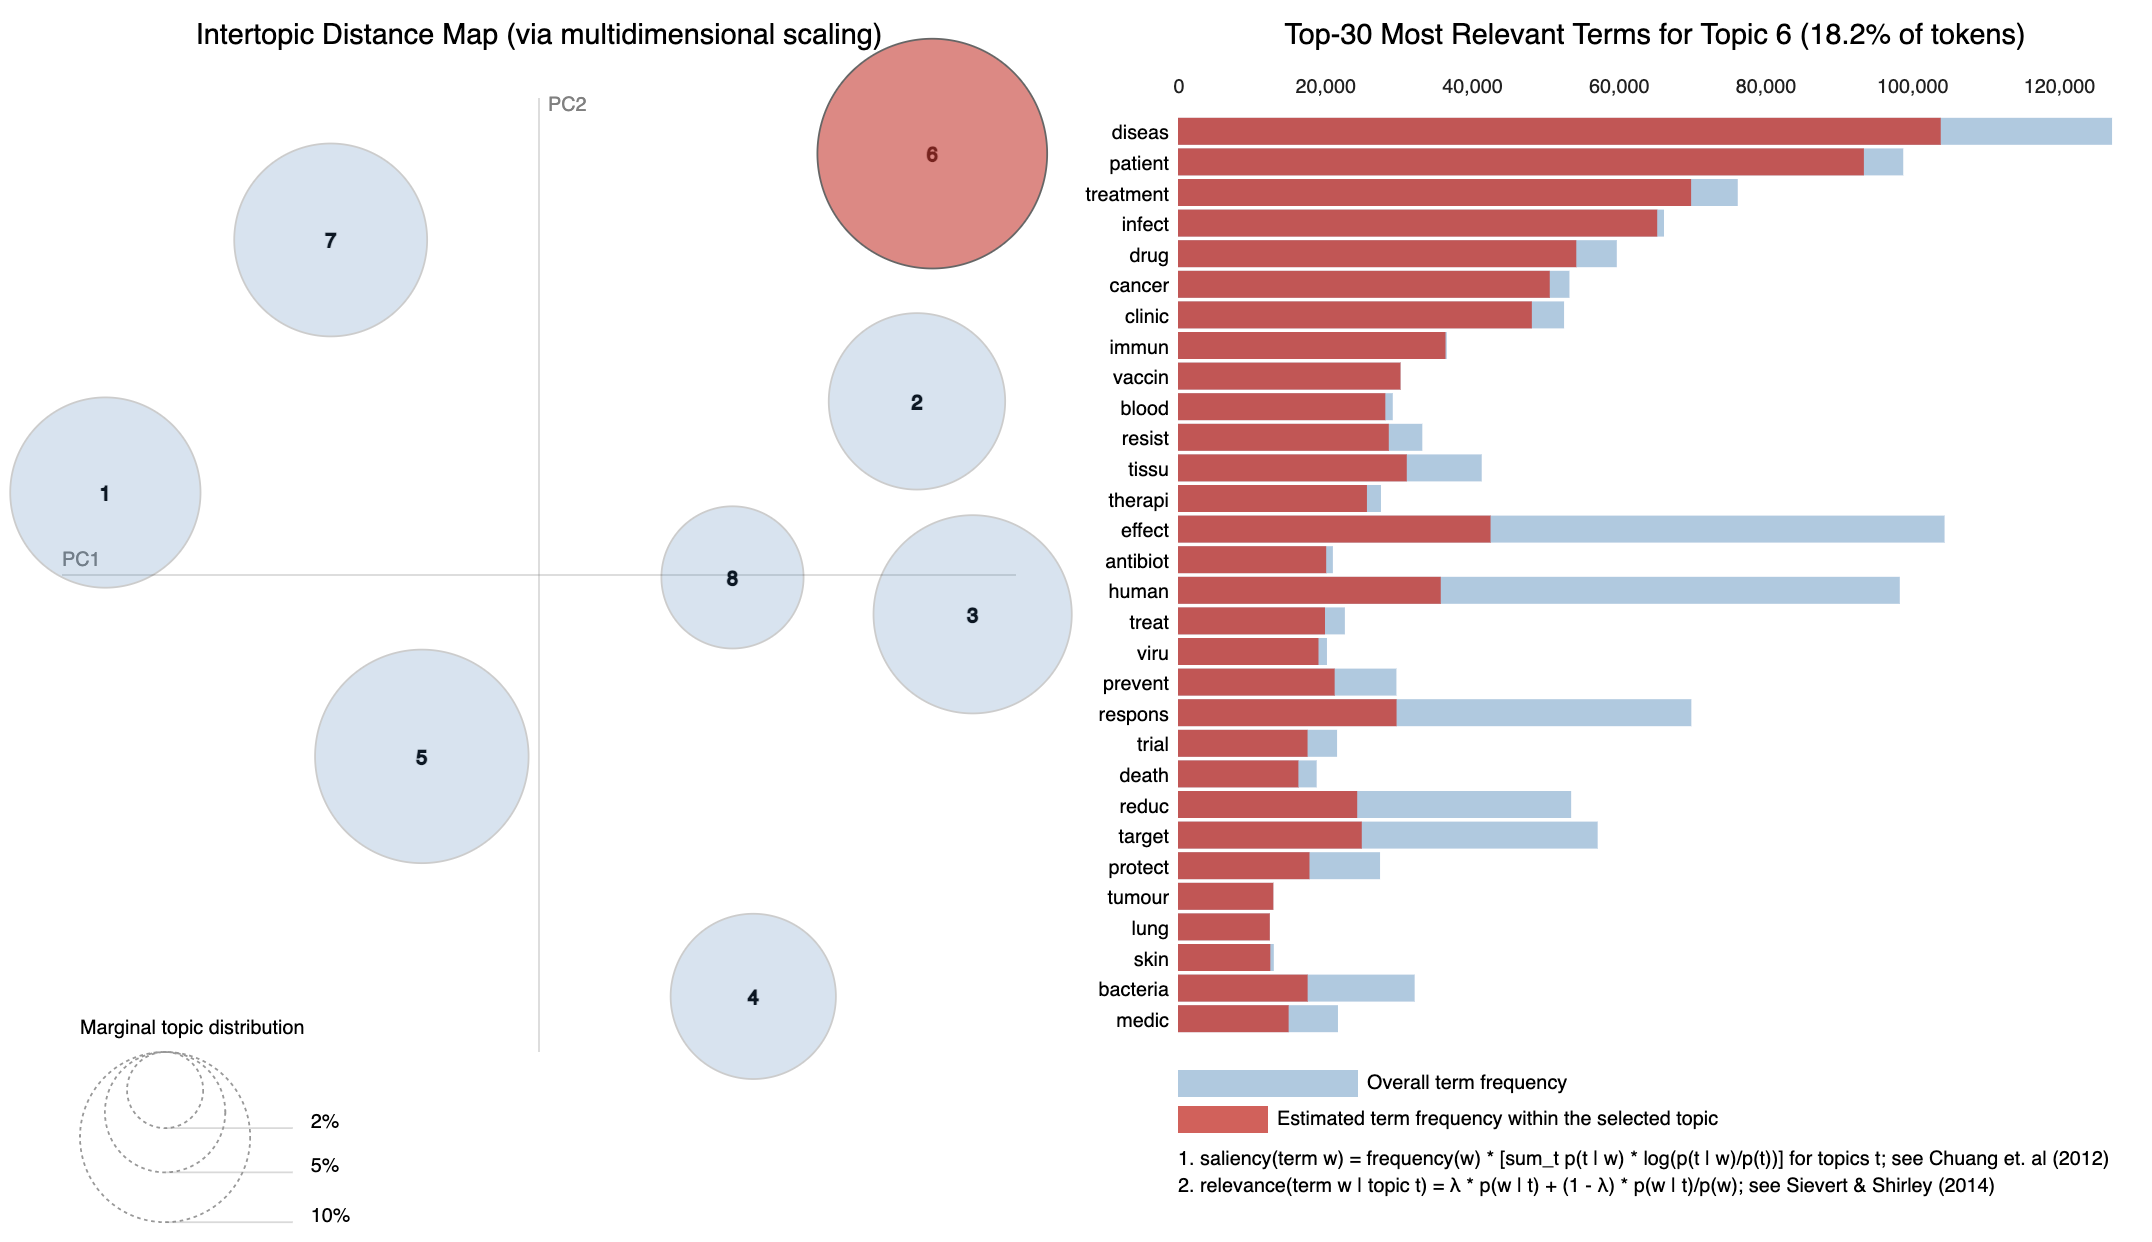
\includegraphics[width = 16cm, height = 10cm]{./img/pylda_topic6.png}
    \caption{Visualisation of topic 6 by pyLDAvis}
\end{figure}

\begin{figure}[H]
    \centering
    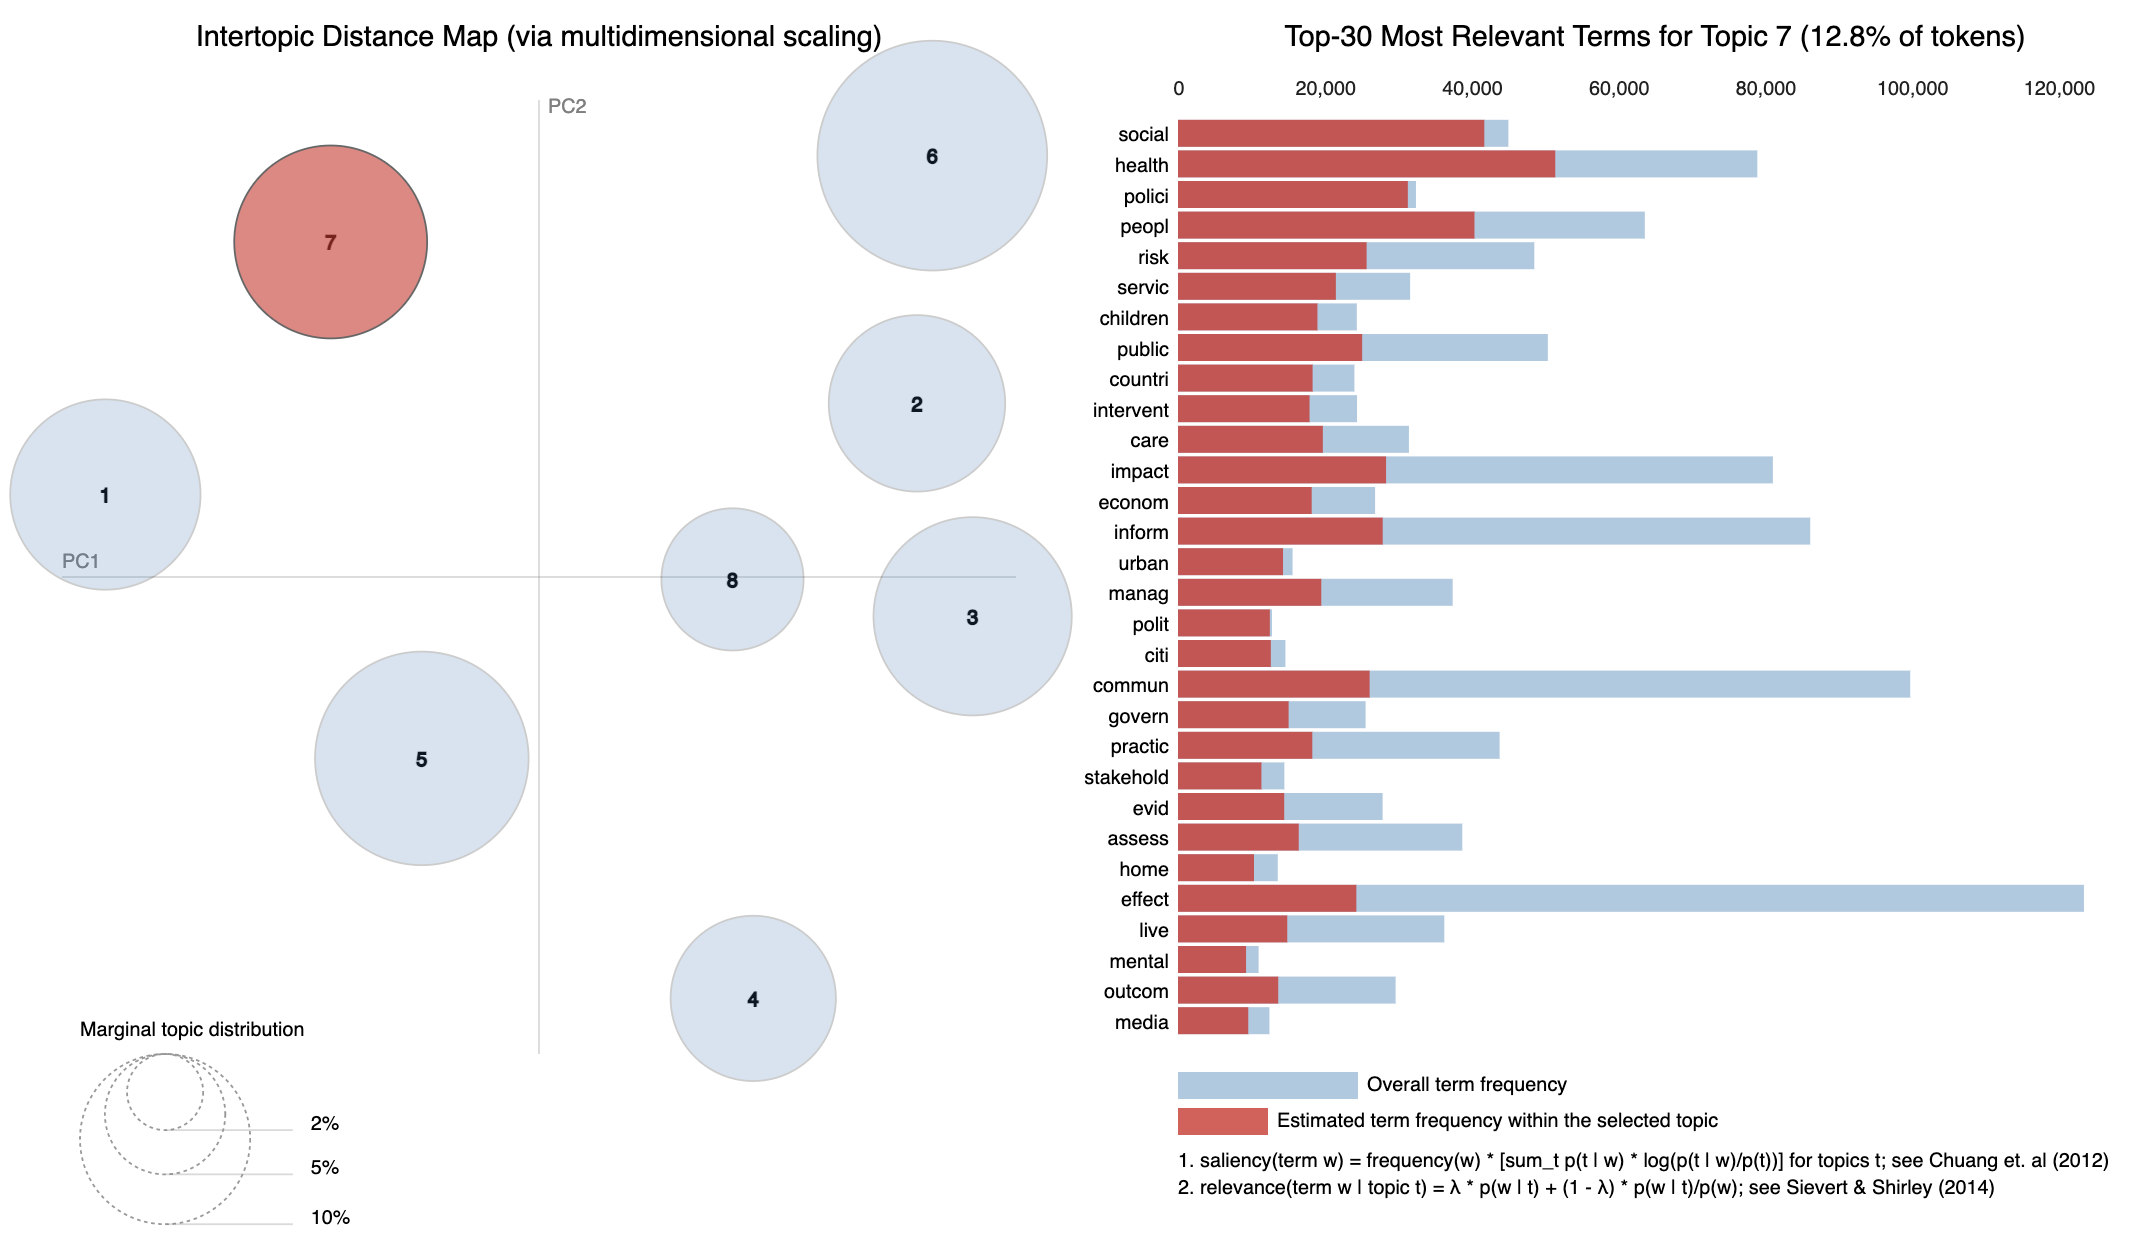
\includegraphics[width = 16cm, height = 10cm]{./img/pylda_topic7.png}
    \caption{Visualisation of topic 7 by pyLDAvis}
\end{figure}

\begin{figure}[H]
    \centering
    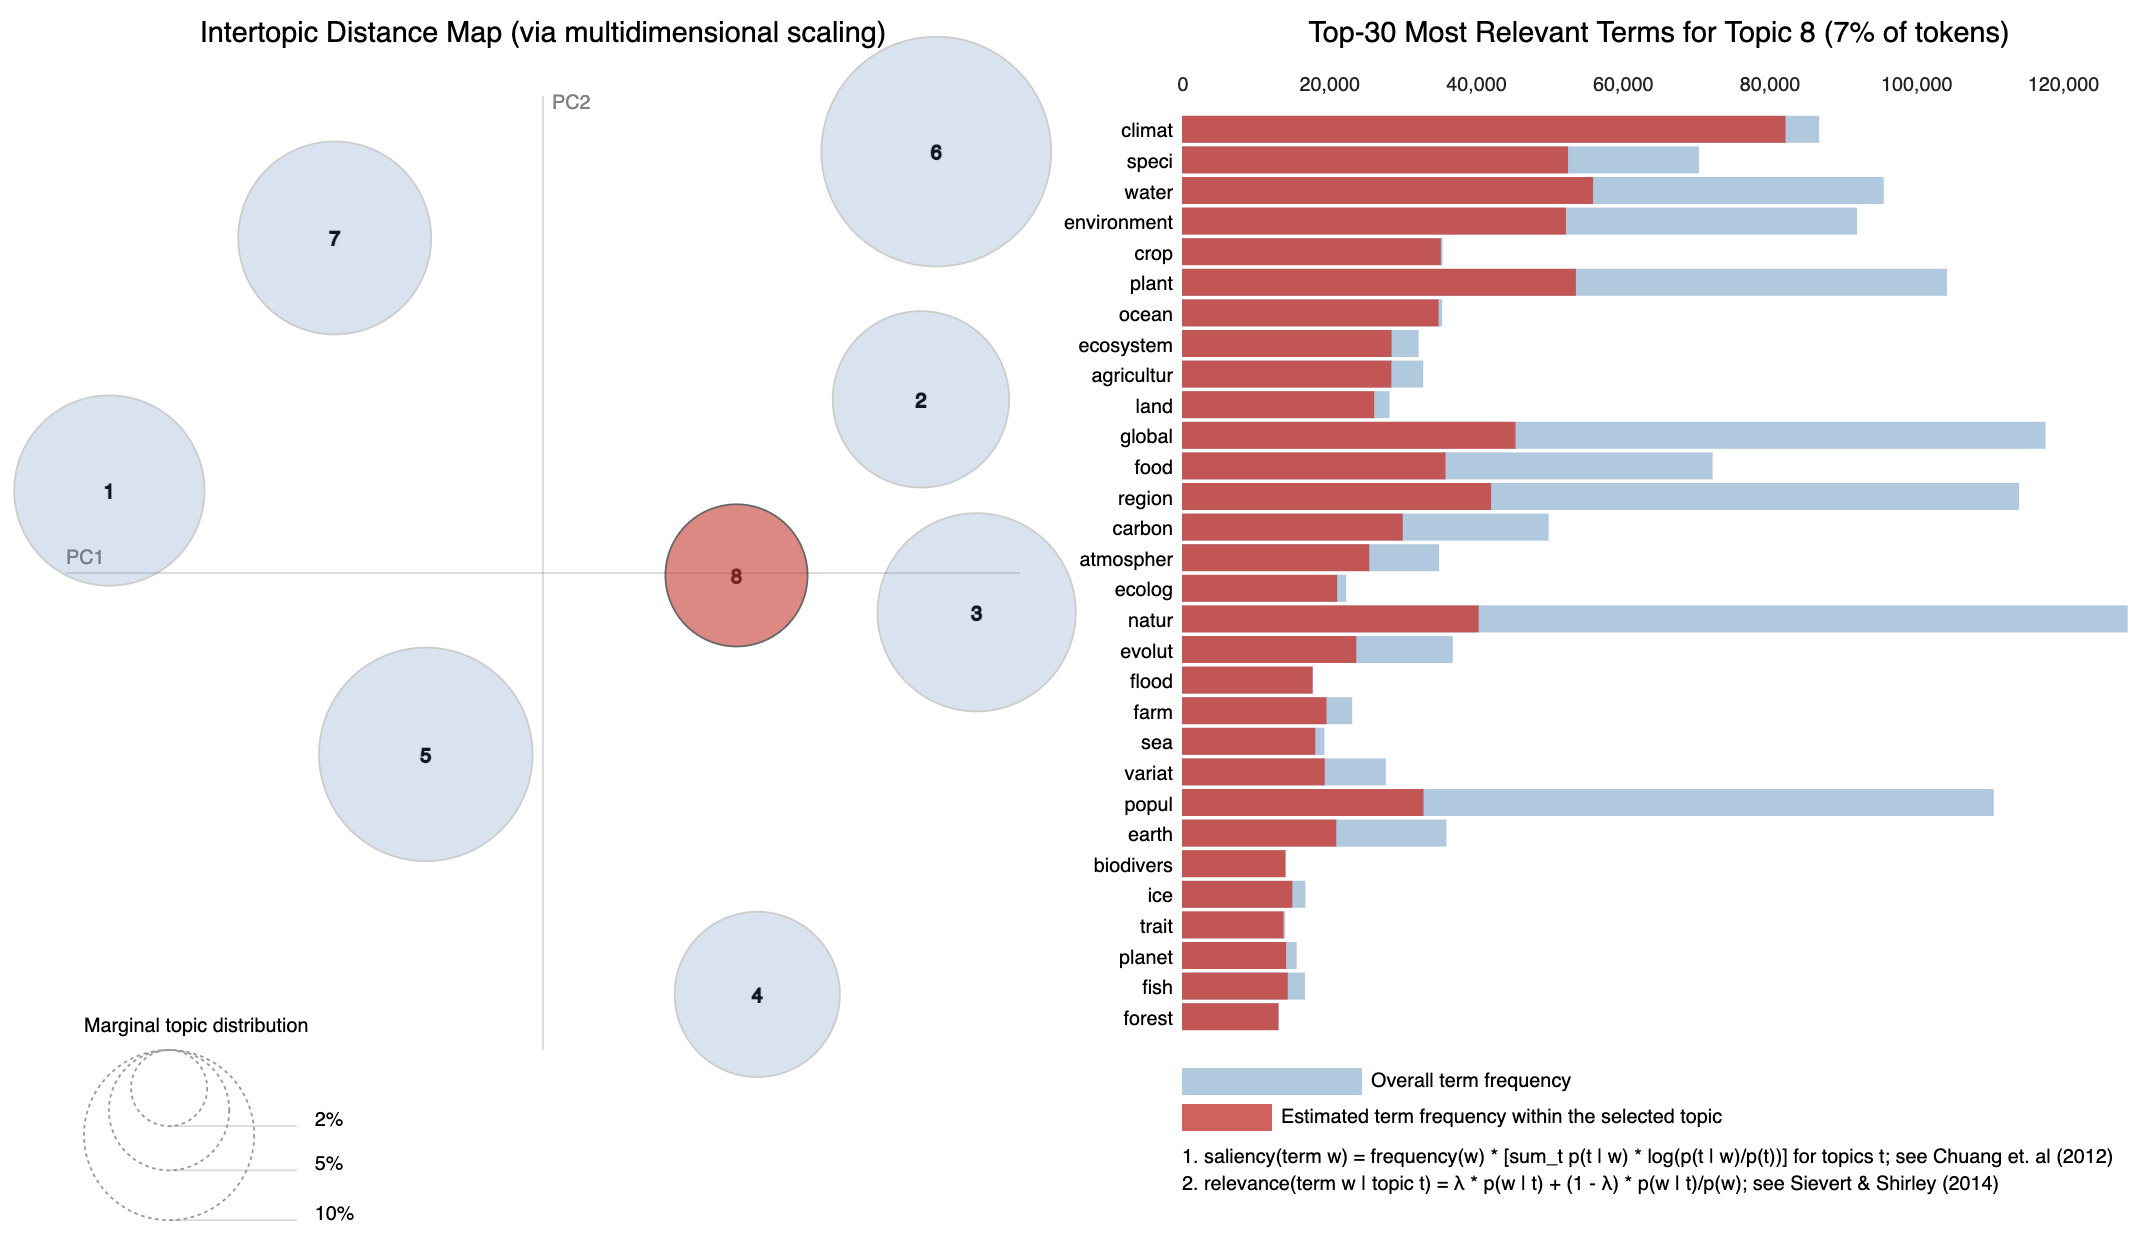
\includegraphics[width = 16cm, height = 10cm]{./img/pylda_topic8.png}
    \caption{Visualisation of topic 8 by pyLDAvis}
\end{figure}

\begin{figure}[H]
    \centering
    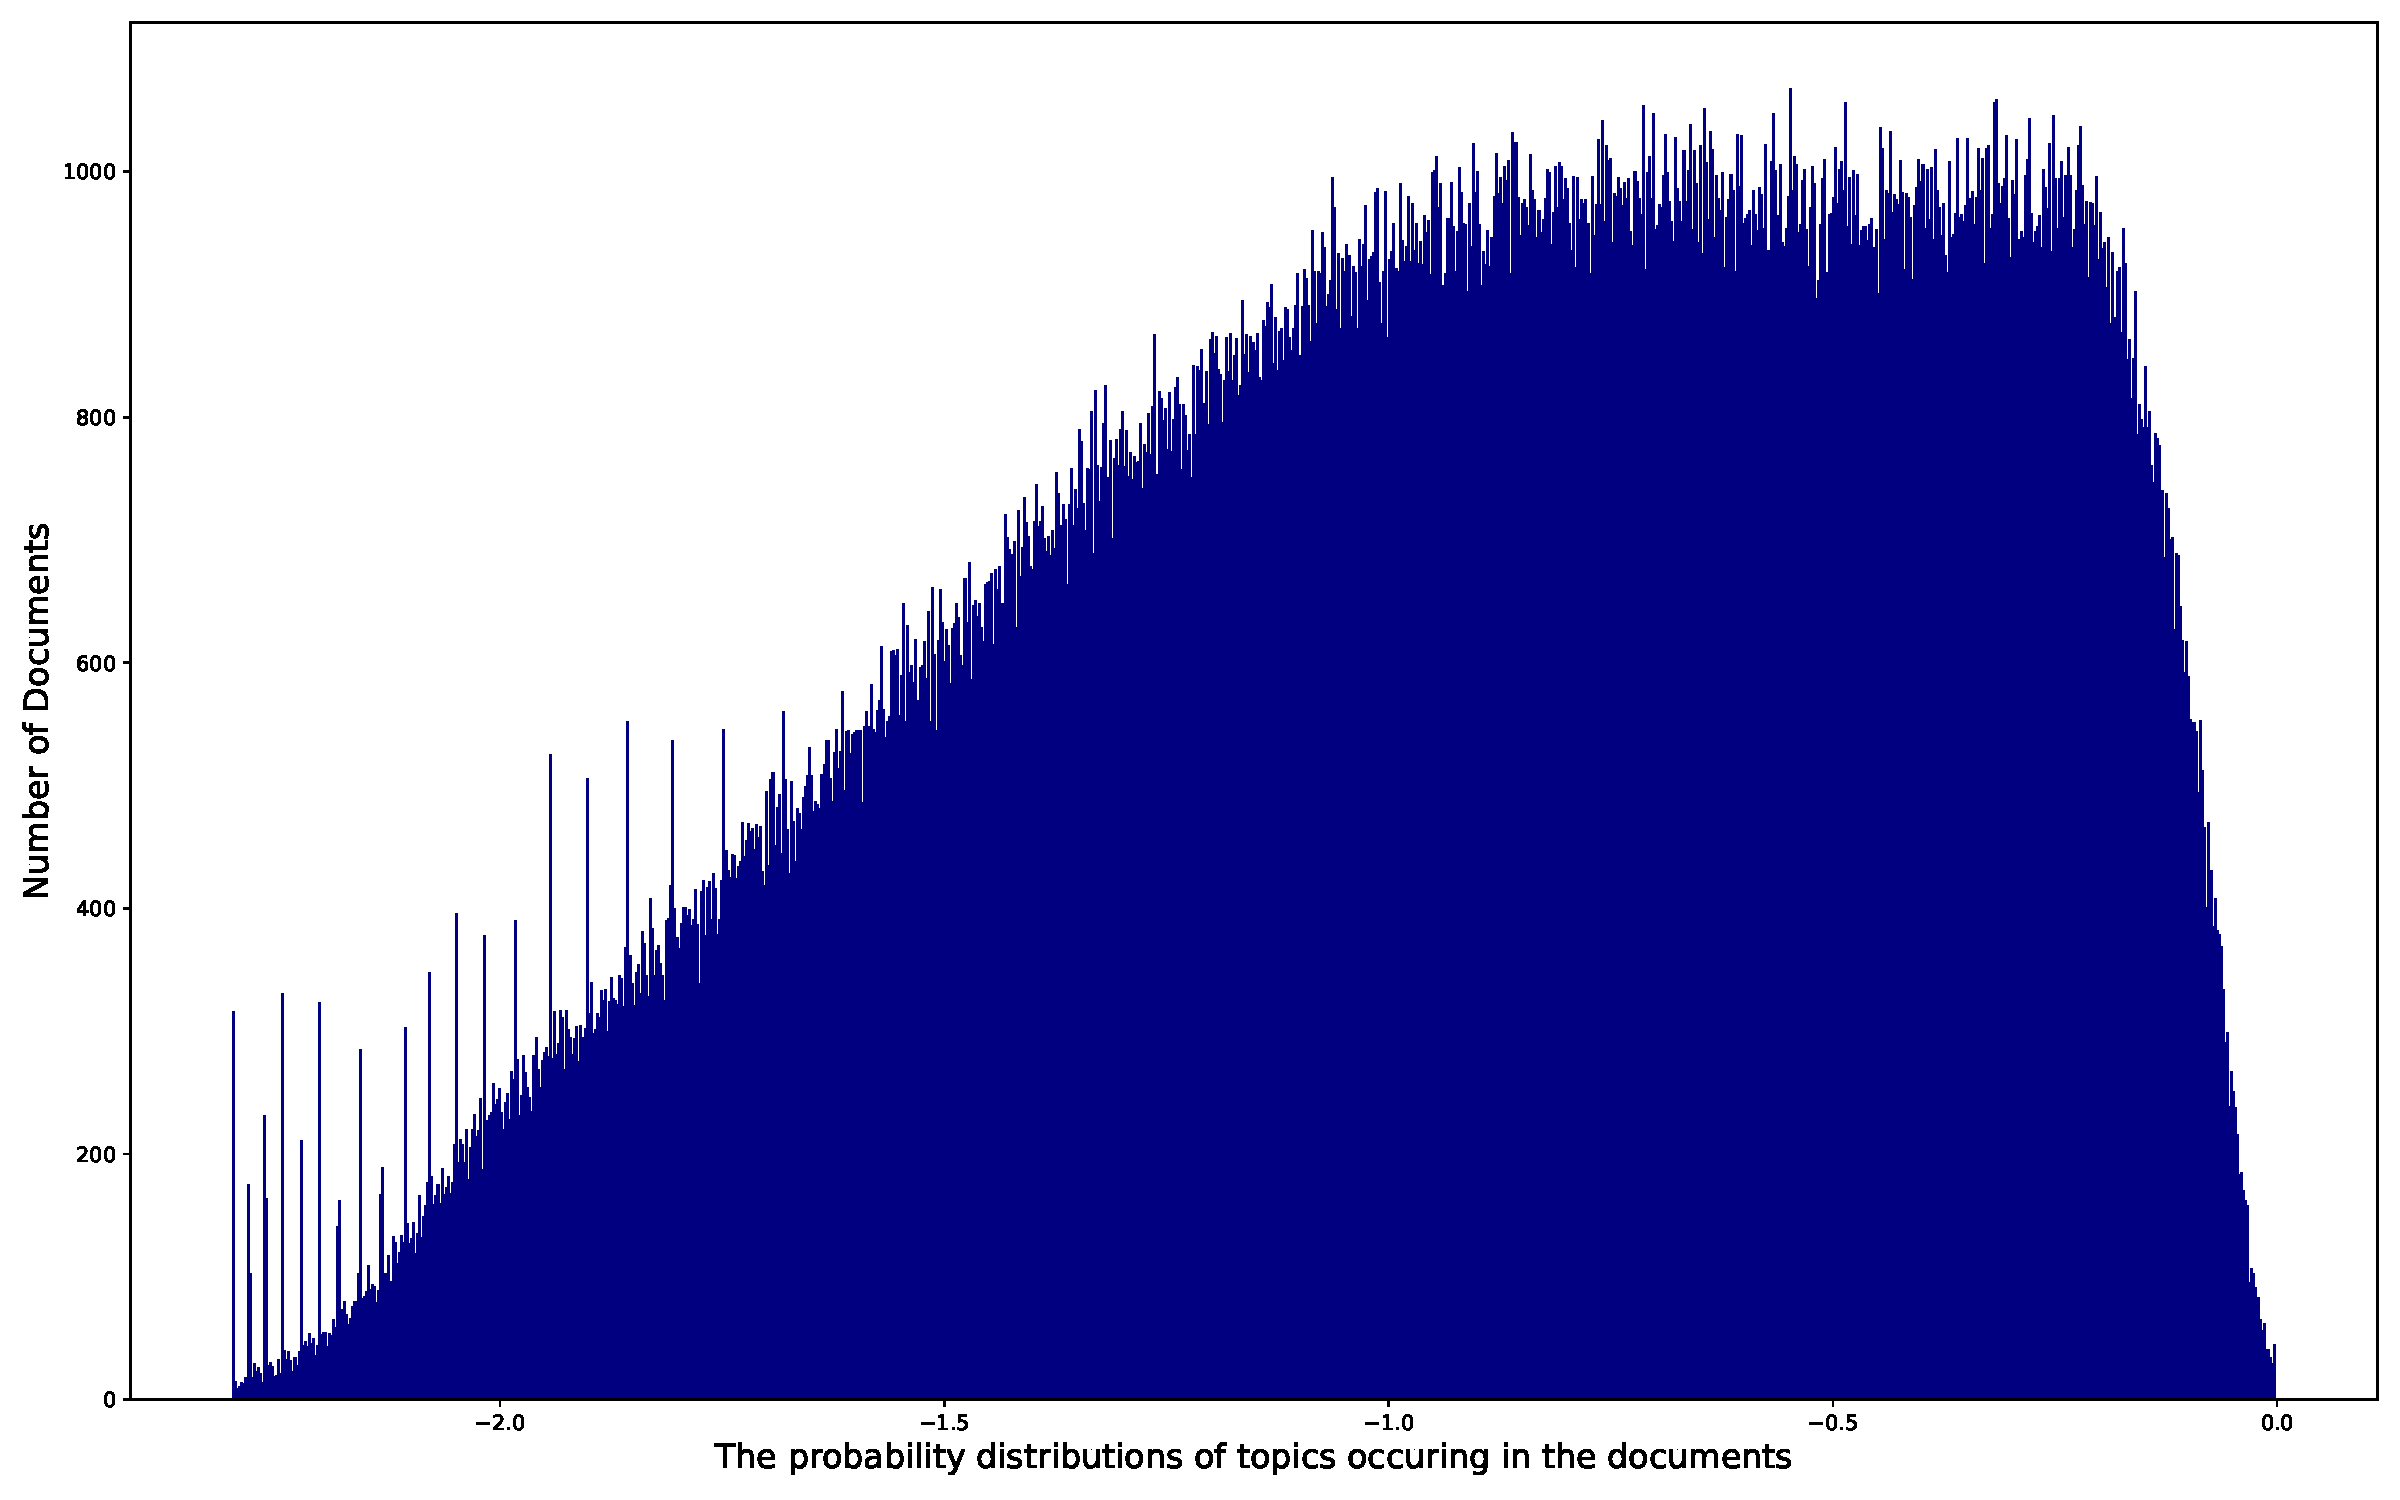
\includegraphics[width = 16cm, height = 9cm]{./img/distri_doc_word_counts_after_cut.pdf}
    \caption[The probability distribution of topic probabilities after cut small probabilities]{The probability distribution of topic probabilities that are more than 0.005 in all documents}
\end{figure}

\begin{figure}[H]
    \centering
    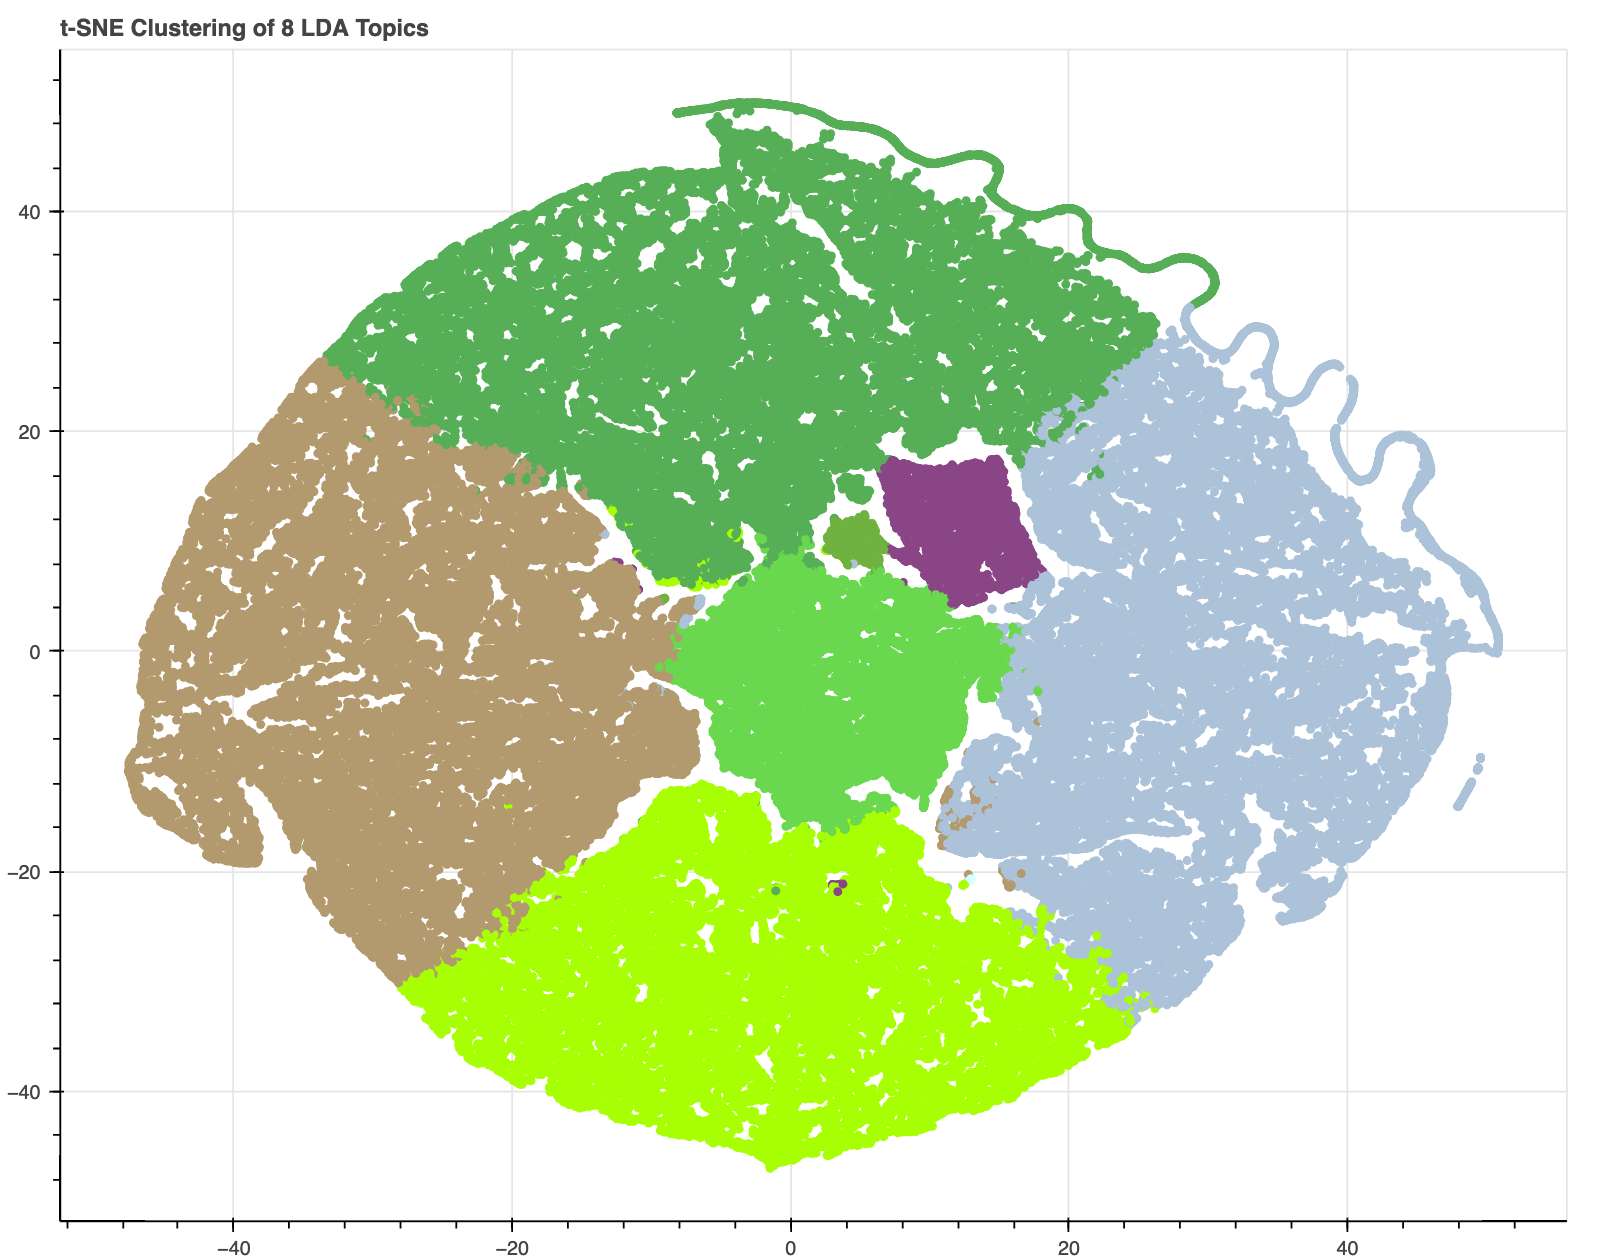
\includegraphics[width = 16cm, height = 12cm]{./img/t-sne.png}
    \caption{t-SNE clustering for visualisation of eight topics}
\end{figure}

% \subsection{Distributions of document word counts by dominant topic}
%
\begin{figure}[H]
    \centering
    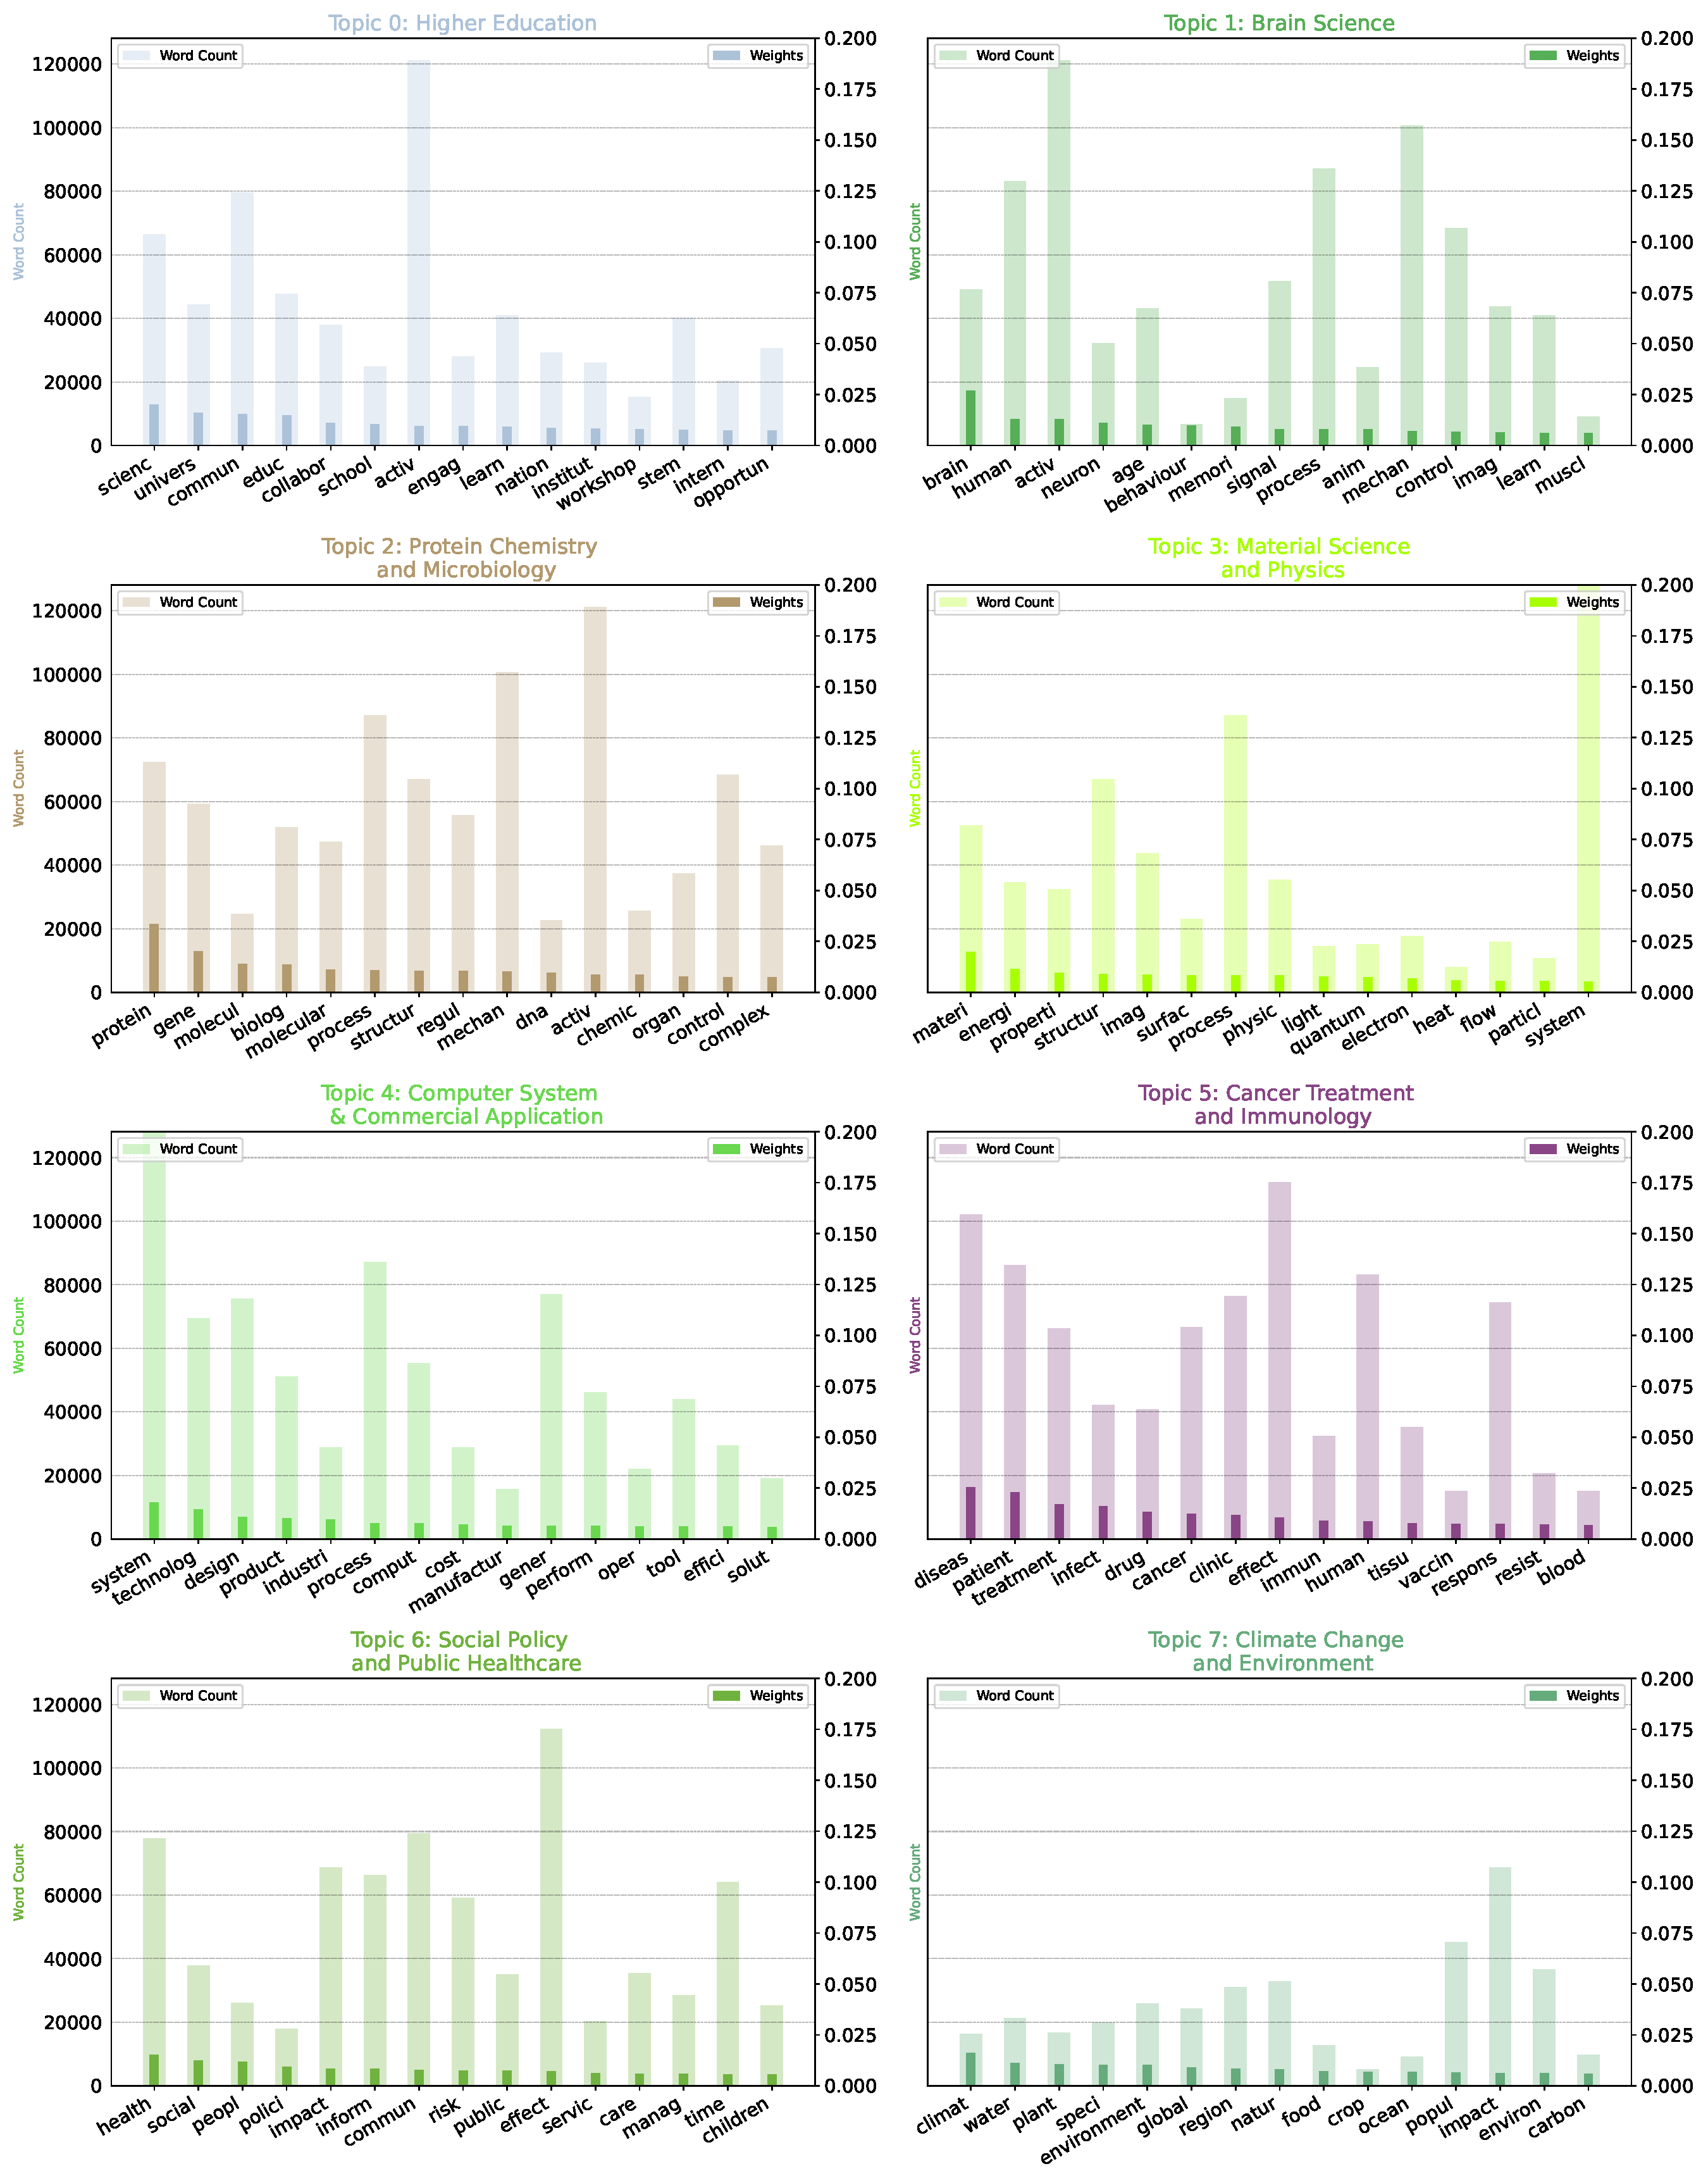
\includegraphics[width = 17cm, height = 24cm]{./img/word_count_and_importance_of_topic_keywords.pdf}
    \caption{Word count and importance of topic keywords}
\end{figure}
%
% \subsection{Sentences coloring of 20 sentences by dominant topic}
%
\begin{figure}[H]
    \centering
    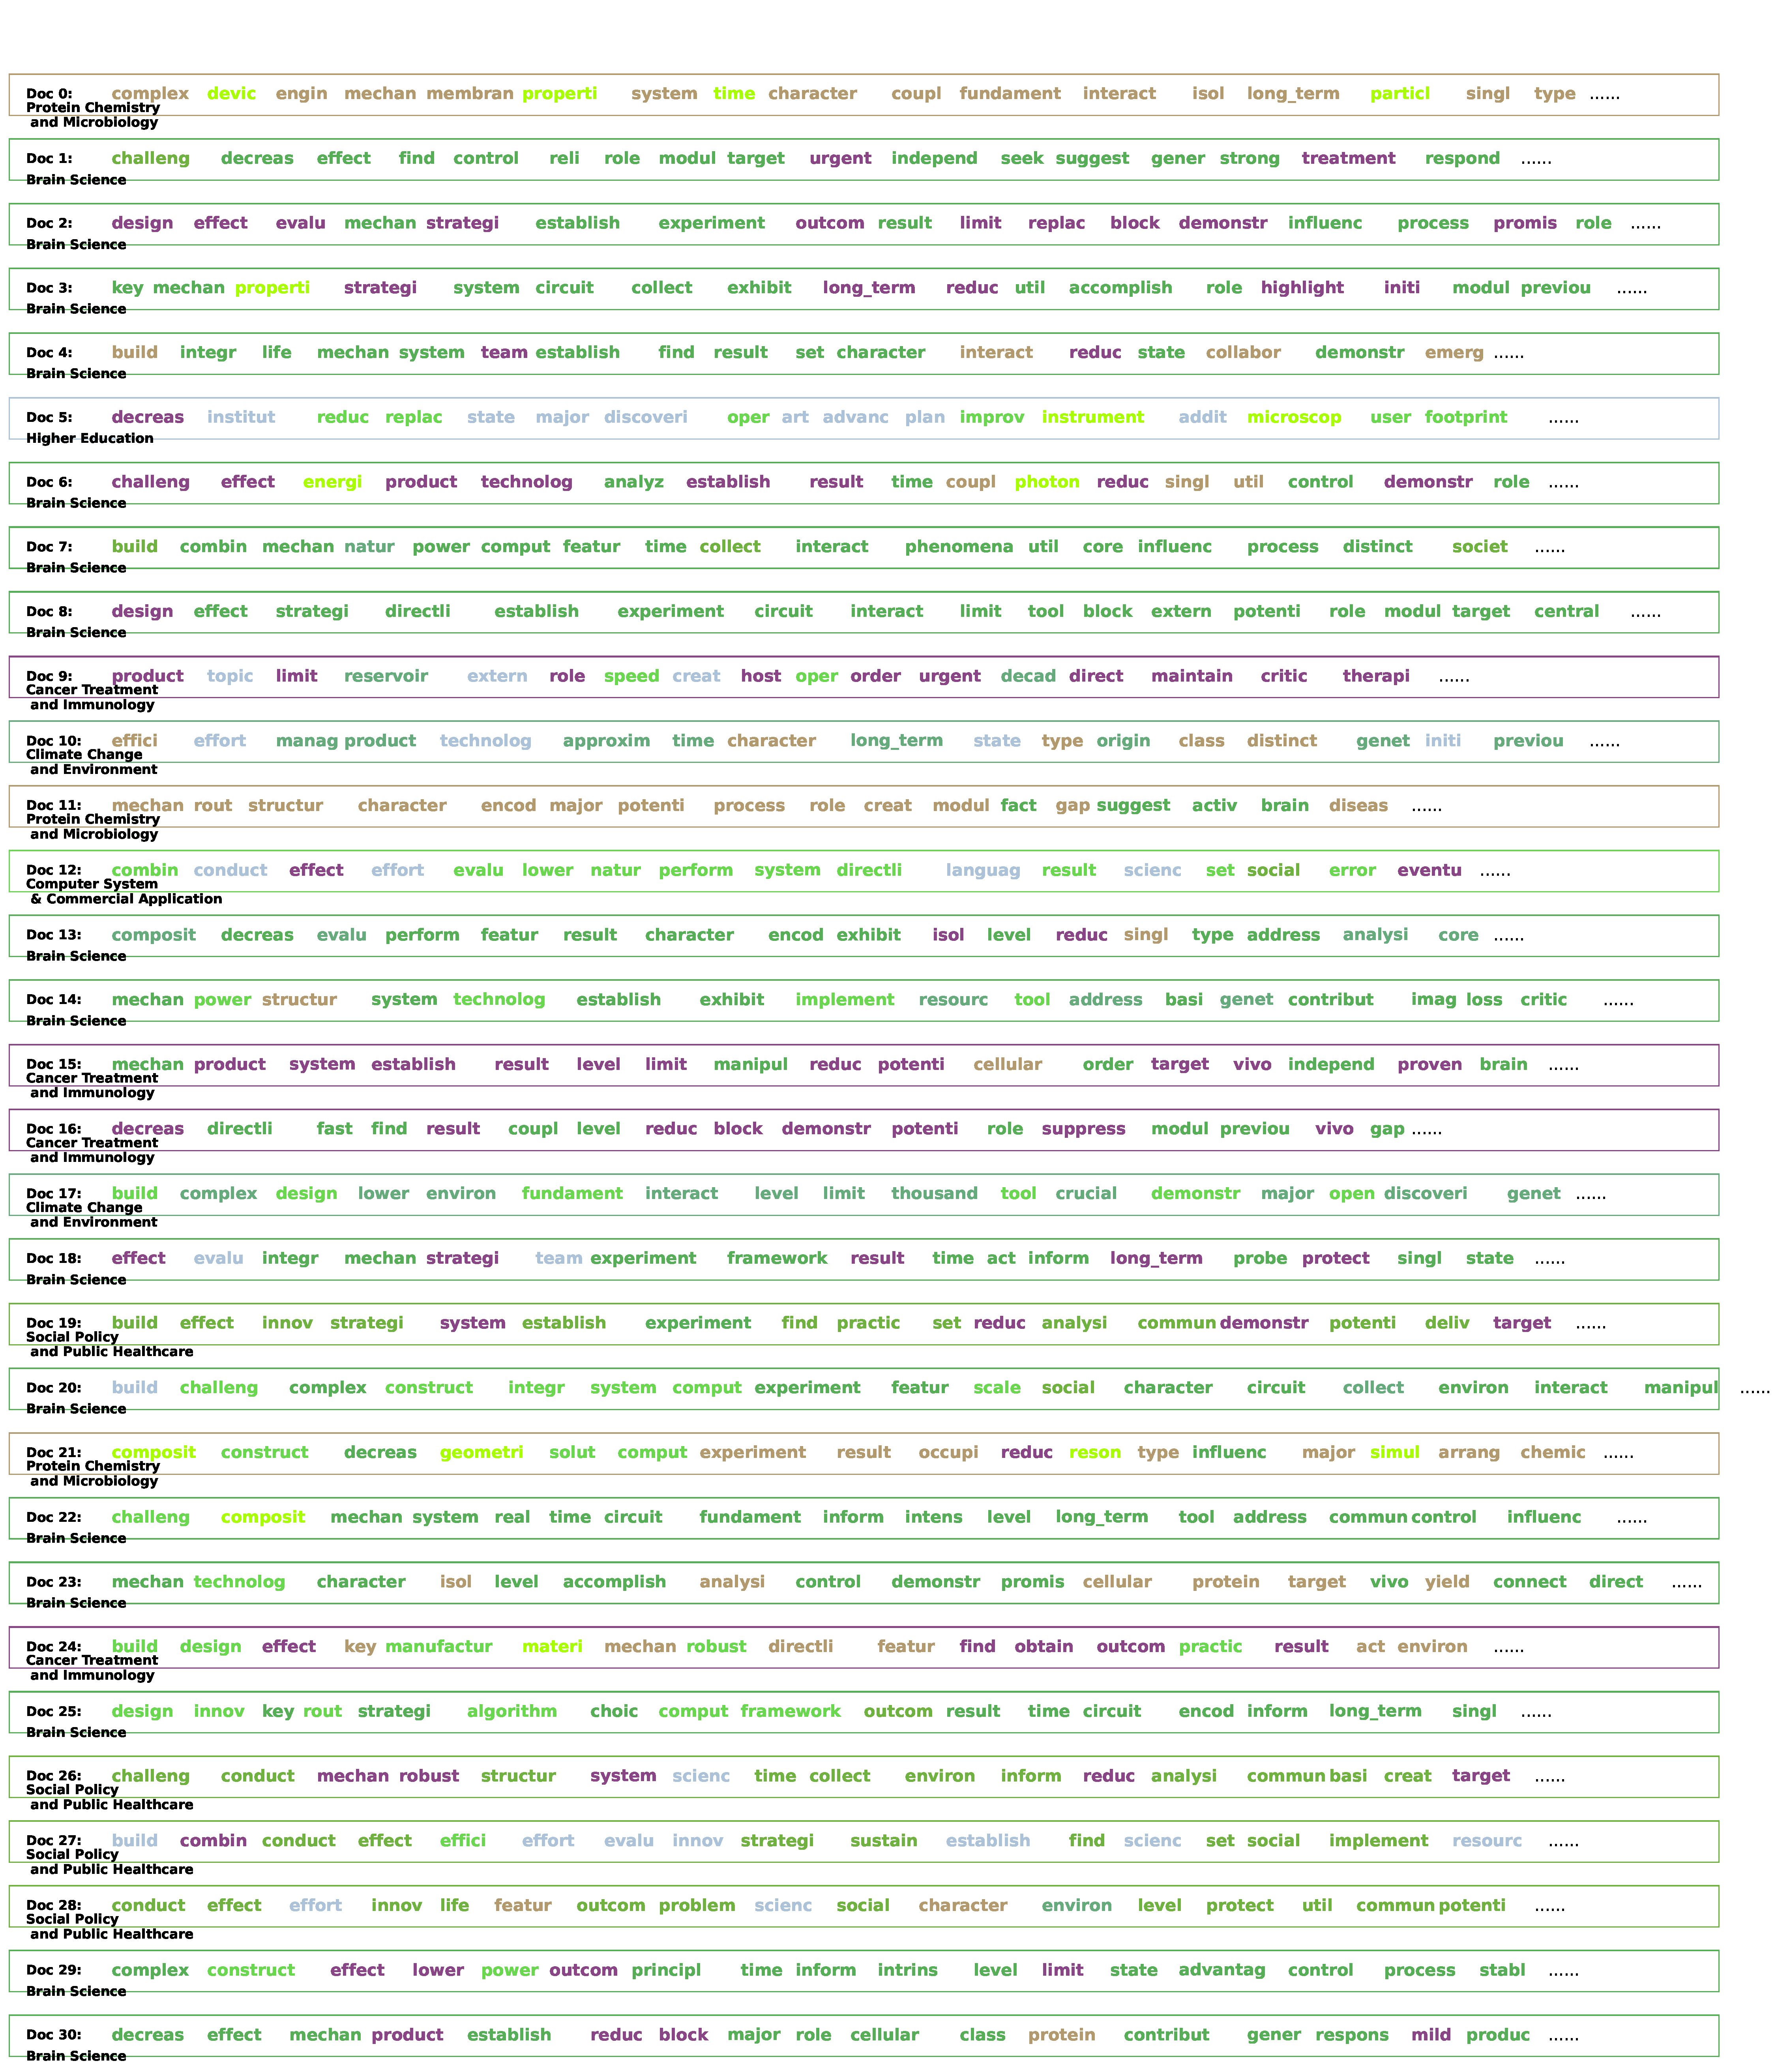
\includegraphics[width = 17cm, height = 24cm]{./img/sentences.pdf}
    \caption{Sentences coloring of dominant topic in part of documents}
\end{figure}
%
% \subsection{t-SNE Clustering of 8 topics}
%


% \newpage
% \bibliographystyle{IEEEtran}
% \bibliography{references}

% \end{document}
